% This header is the default LaTeX template for generating documents with Ampersand.
% It was generated with Ampersand vs. 2.1.0.71
% You can modify this file to make it fit your needs. However, the required knowledge of 
% LaTeX is not documented here. You can find help with that at http://en.wikibooks.org/wiki/LaTeX
% see the ampersand user guide (TODO) for more information on how to apply your own LaTeX header
%
\documentclass[10pt,a4paper]{report}              % Define the document class
\parskip 12pt plus 2.5pt minus 4pt                % Extra vertical space between paragraphs.
\parindent 0em                                    % Width of paragraph indentation.

% -- pachages used for several purposes:
\usepackage{glossary}
\makeglossary
\usepackage{theorem}
\usepackage{amssymb}
\usepackage{amsmath}         % Provides various features to facilitate writing math formulas and to improve the typographical quality of their output.
\usepackage{ucs}             % Provides various features for UTF8 (internationalization) stuff
\usepackage[utf8x]{inputenc} %
\theoremstyle{plain}\theorembodyfont{\rmfamily}\newtheorem{definition}{Definition}[section]
\theoremstyle{plain}\theorembodyfont{\rmfamily}\newtheorem{designrule}[definition]{Requirement}
\usepackage{graphicx}
\def\id#1{\mbox{\em #1\/}}
\newcommand{\marge}[1]{\marginpar{\begin{minipage}[t]{3cm}{\noindent\small\em #1}\end{minipage}}}
\def\define#1{\label{dfn:#1}\index{#1}{\em #1}}
\def\defmar#1{\label{dfn:#1}\index{#1}\marge{#1}{\em #1}}
\newcommand{\iden}{\mathbb{I}}
\newcommand{\ident}[1]{\mathbb{I}_{#1}}
\newcommand{\full}{\mathbb{V}}
\newcommand{\fullt}[1]{\mathbb{V}_{[#1]}}
\newcommand{\flip}[1]{{#1}^\smallsmile} %formerly:  {#1}^\backsim
\newcommand{\kleeneplus}[1]{{#1}^{+}}
\newcommand{\kleenestar}[1]{{#1}^{*}}
\newcommand{\cmpl}[1]{\overline{#1}}
\newcommand{\subs}{\vdash}
\newcommand{\rel}{\times}
\newcommand{\fun}{\rightarrow}
\newcommand{\isa}{\sqsubseteq}
\newcommand{\N}{\mbox{\msb N}}
\newcommand{\disjn}[1]{\id{disjoint}(#1)}
\newcommand{\fsignat}[3]{\id{#1}:\id{#2}\fun\id{#3}}
\newcommand{\signat}[3]{\id{#1}:\id{#2}\rel\id{#3}}
\newcommand{\signt}[2]{\mbox{\({#1}_{[{#2}]}\)}}
\newcommand{\declare}[3]{\id{#1}:\ \id{#2}\rel\id{#3}}
\newcommand{\fdeclare}[3]{\id{#1}:\ \id{#2}\fun\id{#3}}
% =====================================================================================
% == The hyperref package will take care of turning all internal references of your  ==
% == document into hyperlinks. For this to work properly some magic is necessary,    ==
% == so you have to put \usepackage[pdftex]{hyperref} as the last command            ==
% == into the preamble of your document.                                             ==
% == Many options are available to customize the behaviour of the hyperref           ==
% == package. See http://ctan.tug.org/tex-archive/info/lshort/english/lshort.pdf     ==
% =====================================================================================
\usepackage[pdftex,colorlinks=false]{hyperref}
%  -- end of Ampersand specific header. The remainder is PanDoc-specific. run C:>pandoc -D latex  to see the default template.
\setlength{\parindent}{0pt}
\setlength{\parskip}{6pt plus 2pt minus 1pt}
\usepackage{enumerate}
\usepackage{array}
% This is needed because raggedright in table elements redefines \\:
\newcommand{\PreserveBackslash}[1]{\let\temp=\\#1\let\\=\temp}
\let\PBS=\PreserveBackslash

\title{Functional Specification of `VIRO'}
\author{Put author(s) here\\(This document was generated by Ampersand vs. 2.1.0.71)}
\date{Thu May 26 10:14:29 EDT 2011}

\begin{document}
\maketitle

\tableofcontents

\chapter{Introduction}\label{chpIntro}

This document defines the functionality of an information system called `VIRO'. It defines business services in a system where people and applications work together in order to fullfill their commitments. A number of these rules have been used as functional requirement to assemble this functional specification\footnote{To use agreements as functional requirements characterizes the Ampersand approach, which has been used to produce this document. }. Those rules are listed in chapter \ref{chpFunctionalRequirements}, ordered by theme. 

The diagnosis in chapter \ref{chpDiagnosis} is meant to help the authors identify shortcomings in their Ampersand script.

The conceptual analysis in chapter \ref{chpConceptualAnalysis} is meant for requirements engineers and architects to validate and formalize the requirements from chapter \ref{chpFunctionalRequirements}. It is also meant for testers to come up with correct test cases. The formalization in this chapter makes consistency of the functional specification provable. It also yields an unambiguous interpretation of all requirements.

Chapters that follow have the builders of `VIRO' as their intended audience. The data analysis in chapter \ref{chpDataAnalysis} describes the data sets upon which `VIRO' is built. Each subsequent chapter defines one business service. This allows builders focus on a single service at a time. Together, these services fulfill all commitments from chapter \ref{chpFunctionalRequirements}. By disclosing all functionality exclusively through these services, `VIRO' ensures compliance to all rules from chapter \ref{chpFunctionalRequirements}. 

\chapter{Shared Language}\label{chpFunctionalRequirements}

This chapter defines the natural language, in which functional requirements of `VIRO' can be discussed and expressed. The purpose of this chapter is to create shared understanding among stakeholders. The language of `VIRO' consists of concepts and basic sentences. All functional requirements are expressed in these terms. When stakeholders can agree upon this language, at least within the scope of `VIRO', they share precisely enough language to have meaningful discussions about functional requirements. All definitions have been numbered for the sake of traceability. 

\section{CaseRegistration}

The registration of administrative cases is based on three articles from
the Dutch administrative law, 'Algemene wet bestuursrecht (Awb)'. An
administrative case is a legal case against a decision of an
administrative authority. Within the 'VIRO' context the terms 'case' and
'legal case' will always refer to an administrative case.

Article 1:1 Awb

\begin{enumerate}[1.]
\item
  'Administrative authority' means:
\end{enumerate}
\begin{quote}
\begin{enumerate}[a.]
\item
  an organ of a juristic person governed by public law, or
\item
  any other person or body vested with public authority.
\end{enumerate}
\end{quote}
Article 6:4 Awb

\begin{enumerate}[1.]
\item
  An objection is lodged by filing a notice of objection with the
  administrative authority which took the decision.
\item
  An administrative appeal is lodged by filing a notice of appeal with
  an appellate authority.
\item
  An appeal to an administrative court is lodged by filing a notice of
  appeal with that court.
\end{enumerate}
Article 8:24 Awb

\begin{enumerate}[1.]
\item
  A party may be assisted or represented by an authorized
  representative.
\item
  The district court may require written authorization of a
  representative.
\item
  Paragraph 2 does not apply to members of the Dutch Bar.
\end{enumerate}
Notices as referred to in art.6:4 Awb are filed in the case file.
Written authorizations as referred to in 8:24 par.3 Awb are filed in the
case file.

\begin{description}
\item[Requirement 1 (rule@line70):]
\label{ReqRule:rule@line70}
The plaintiff in an administrative case is a juristic person

\end{description}
\begin{description}
\item[Requirement 2 (rule@line73):]
\label{ReqRule:rule@line73}
The defendant in an administrative case is an administrative authority
as referred to in art.1:1 Awb.

\end{description}
\begin{description}
\item[Requirement 3 (rule@line84):]
\label{ReqRule:rule@line84}
Written authorizations for representatives of a case are not put in the
case file

\end{description}
\begin{description}
\item[Requirement 4 (rule@line92):]
\label{ReqRule:rule@line92}
Every administrative case is either an appeal or an objection or an
appeal to an administrative court. (Art.6:4 Awb)

\end{description}
\begin{description}
\item[Requirement 5 (rule@line103):]
\label{ReqRule:rule@line103}
Every party is either a person or an organization or an administrative
authority.

\end{description}
\begin{description}
\item[Requirement 6 (rule@line107):]
\label{ReqRule:rule@line107}
Members of the government, i.e., Ministers and Secretaries of State, are
administrative authorities according to the constitution.

\end{description}
\section{Sessions}

When administrative cases are brought before the district court, they
are assigned to a scheduled session with a certain panel of judges. The
registration of sessions is based on article 8:10 Awb.

Article 8:10 Awb

\begin{enumerate}[1.]
\item
  Cases brought before the district court shall first be considered by a
  single-judge panel.
\item
  If the single-judge panel deems a case unsuitable for consideration by
  a single judge, it will refer it to a three-judge panel. A
  single-judge panel may also refer a case to a three-judge panel for
  other reasons.
\item
  If a three-judge panel thinks that a case is suitable for further
  consideration by a single judge, it may refer it to a single-judge
  panel.
\item
  A case may be referred at any stage of the proceedings. The case shall
  then be resumed at the point at which it was referred.
\end{enumerate}
The organization of panels is defined in the Dutch law for the
administration of justice, 'Wet op de rechterlijke organisatie (RO)'.
For example article 6:1 RO describes that there are single-judge and
three-judge panels, of which the members are recognized judges. Article
41 par.1 RO defines that the district court is seated in the main city
of the jurisdiction. Article 41 par.2 RO allows for local offices of the
district court.

For illustration purposes, article 8:7 par.1 Awb will be maintained
within the 'VIRO' context.

\begin{description}
\item[Requirement 7 (rule@line123):]
\label{ReqRule:rule@line123}
a session can be identified by its panel, its city and its date.

\end{description}
\begin{description}
\item[Requirement 8 (rule@line135):]
\label{ReqRule:rule@line135}
A judge at a session is a member of the panel that runs the session.

\end{description}
\begin{description}
\item[Requirement 9 (rule@line137):]
\label{ReqRule:rule@line137}
The clerk of a session must be the clerk of the court where the session
is held.

\end{description}
\begin{description}
\item[Requirement 10 (rule@line143):]
\label{ReqRule:rule@line143}
All sessions are scheduled

\end{description}
\begin{description}
\item[Requirement 11 (rule@line149):]
\label{ReqRule:rule@line149}
Administrative authorities as referred to in art.8:7 par.1 Awb are
administrative authorities as referred to in art.1:1 Awb.

\end{description}
\begin{description}
\item[Requirement 12 (rule@line151):]
\label{ReqRule:rule@line151}
An appeal lodged against a decision of an administrative authority of a
province or municipality, or a water management board, or a region as
referred to in article 21 of the 1993 Police Act, or of a joint body or
public body established under the Joint Arrangements Act, falls within
the jurisdiction of the district court within whose district the
administrative authority has its seat. (art. 8:7 par.1 Awb.)

\end{description}
\section{CaseFiles}

This paragraph describes the theme `CaseFiles'.

\begin{description}
\item[Requirement 13 (file documents):]
\label{ReqRule:file documents}
Documents are put in a case file except for written authorizations for
representatives.

\end{description}
\section{Scheduling}

This paragraph describes the theme `Scheduling'.

\begin{description}
\item[Requirement 14 (assign cases):]
\label{ReqRule:assign cases}
Cases must be assigned to a process in a scheduled session.

\end{description}
\chapter{Diagnosis}\label{chpDiagnosis}

This chapter provides an analysis of the Ampersand script of `VIRO'. This analysis is intended for the authors of this script. It can be used to complete the script or to improve possible flaws. 

VIRO does not specify which roles may change the contents of which relations. 
VIRO assigns rules to roles. The following table shows the rules that are being maintained by a given role.

\begin{center}
\begin{tabular}{lcc}
rule & Archivist & Scheduler\\
\hline
file documents & $\times$ & \\
assign cases &  & $\times$\\
\end{tabular}
\end{center}

Concepts Party, LegalCase, City, Document, AreaOfLaw, DocumentType, CaseType, Process, Session, Panel, Court, Role, Date, CourtOfAppeal, TimeStamp, and Text remain without a definition.

The purpose of relations ${\id{caseFile}}$, ${\id{documentType}}$, ${\id{remark}}$, ${\id{sent}}$, ${\id{received}}$, ${\id{areaOfLaw}}$, ${\id{caseType}}$, ${\id{objection}}$, ${\id{appealToAdminCourt}}$, ${\id{appeal}}$, ${\id{writtenAuthOf}}$, ${\id{plaintiff}}$, ${\id{authFor}}$, ${\id{authBy}}$, ${\id{defendant}}$, ${\id{legalCase}}$, ${\id{session}}$, ${\id{panel}}$, ${\id{scheduled}}$, ${\id{judge}}$, ${\id{clerk}}_{[{\id{Session}}{\times}{\id{Party}}]}$, ${\id{broughtBefore}}$, ${\id{location}}$, ${\id{seatedIn}}_{[{\id{Court}}{\times}{\id{City}}]}$, ${\id{occured}}$, ${\id{jurisdiction}}$, ${\id{district}}$, ${\id{court}}$, ${\id{members}}$, ${\id{clerk}}_{[{\id{Court}}{\times}{\id{Party}}]}$, ${\id{localOffices}}$, ${\id{actsas}}$, ${\id{organization}}$, ${\id{person}}$, ${\id{administrativeAuthority}}$, ${\id{memberOfGovernment}}$, ${\id{administrativeAuthorityAwb87}}$, and ${\id{domicile}}$ is not documented.

Relations ${\id{writtenAuthOf}}$, ${\id{authBy}}$, ${\id{areaOfLaw}}$, ${\id{documentType}}$, ${\id{caseType}}$, ${\id{session}}$, ${\id{court}}$, ${\id{actsas}}$, ${\id{seatedIn}}_{[{\id{Court}}{\times}{\id{City}}]}$, ${\id{seatedIn}}_{[{\id{CourtOfAppeal}}{\times}{\id{City}}]}$, ${\id{district}}$, ${\id{localOffices}}$, ${\id{sent}}$, ${\id{received}}$, and ${\id{remark}}$ are not used in any rule. 

Figure \ref{fig:LatCaseRegistration} shows a conceptual diagram with all relations declared in `CaseRegistration'.

\begin{figure}[htb]
\begin{center}
\scalebox{.3}[.3]{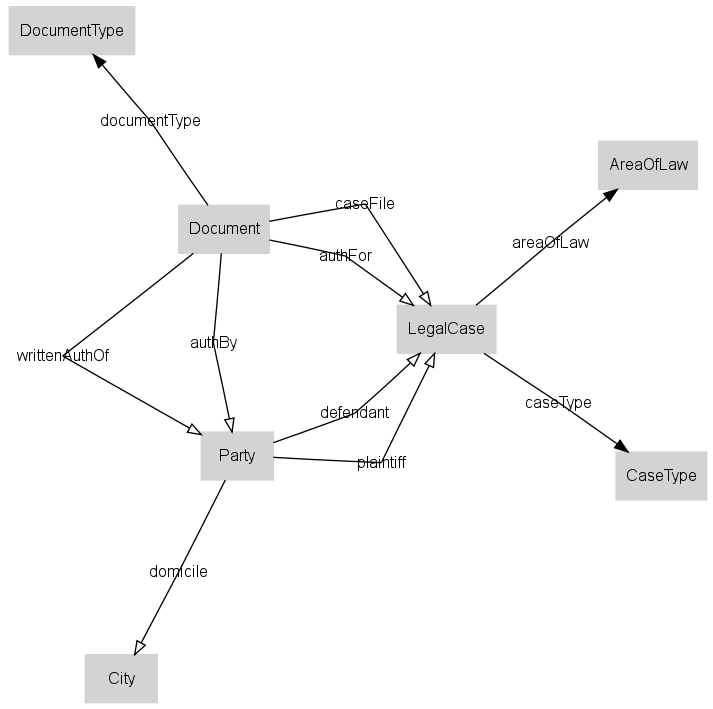
\includegraphics{LatCaseRegistration}}
\caption{Concept analysis of relations in CaseRegistration}
\label{fig:LatCaseRegistration}
\end{center}
\end{figure}
Figure \ref{fig:LatCorrespondence} shows a conceptual diagram with all relations declared in `Correspondence'.

\begin{figure}[htb]
\begin{center}
\scalebox{.3}[.3]{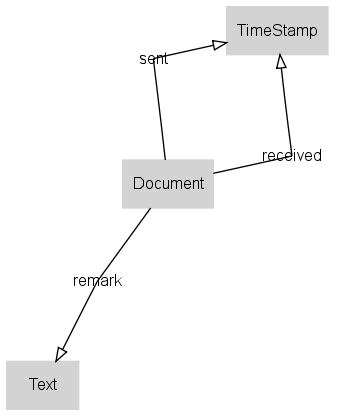
\includegraphics{LatCorrespondence}}
\caption{Concept analysis of relations in Correspondence}
\label{fig:LatCorrespondence}
\end{center}
\end{figure}
On line numbers line 70, file "fsVIROENG.adl", line 73, file "fsVIROENG.adl", line 84, file "fsVIROENG.adl", line 92, file "fsVIROENG.adl", line 103, file "fsVIROENG.adl", line 107, file "fsVIROENG.adl", line 123, file "fsVIROENG.adl", line 135, file "fsVIROENG.adl", line 137, file "fsVIROENG.adl", line 143, file "fsVIROENG.adl", line 149, file "fsVIROENG.adl", line 151, file "fsVIROENG.adl", line 112, file "fsVIROENG.adl", and line 163, file "fsVIROENG.adl" of file fsVIROENG.adl, rules are defined without a proper explanation of their purpose. 

All rules in all processes are linked to roles.

The role-rule assignments in any of the described processes have been assigned to rules within that same process.

The following table represents the population of various relations. 

\begin{center}
\begin{tabular}{lr}
Concept & Population\\
\hline
Party & 38\\
LegalCase & 3\\
City & 59\\
Document & 10\\
AreaOfLaw & 1\\
DocumentType & 5\\
CaseType & 2\\
Process & 3\\
Session & 4\\
Panel & 7\\
Court & 20\\
Role & 7\\
Date & 4\\
CourtOfAppeal & 6\\
TimeStamp & 18\\
Text & 10\\
\end{tabular}
\end{center}

\begin{center}
\begin{tabular}{lr}
Relation & Population\\
\hline
$\declare{plaintiff}{Party}{LegalCase}$ & 3\\
$\declare{defendant}{Party}{LegalCase}$ & 3\\
$\declare{domicile}{Party}{City}$ & 4\\
$\declare{writtenAuthOf}{Document}{Party}$ & 5\\
$\declare{authFor}{Document}{LegalCase}$ & 4\\
$\declare{authBy}{Document}{Party}$ & 4\\
$\declare{areaOfLaw}{LegalCase}{AreaOfLaw}$ & 3\\
$\declare{caseFile}{Document}{LegalCase}$ & 5\\
$\declare{documentType}{Document}{DocumentType}$ & 10\\
$\declare{caseType}{LegalCase}{CaseType}$ & 3\\
$\declare{appeal}{LegalCase}{LegalCase}$ & 2\\
$\declare{appealToAdminCourt}{LegalCase}{LegalCase}$ & 1\\
$\declare{person}{Party}{Party}$ & 33\\
$\declare{organization}{Party}{Party}$ & 2\\
$\declare{administrativeAuthority}{Party}{Party}$ & 3\\
$\declare{memberOfGovernment}{Party}{Party}$ & 1\\
$\declare{session}{Process}{Session}$ & 3\\
$\declare{legalCase}{Process}{LegalCase}$ & 3\\
$\declare{panel}{Session}{Panel}$ & 4\\
$\declare{court}{Panel}{Court}$ & 7\\
$\declare{members}{Party}{Panel}$ & 14\\
$\declare{judge}{Session}{Party}$ & 4\\
$\declare{clerk}{Session}{Party}$ & 4\\
$\declare{clerk}{Court}{Party}$ & 4\\
$\declare{actsas}{Party}{Role}$ & 38\\
$\declare{broughtBefore}{LegalCase}{Court}$ & 3\\
$\declare{scheduled}{Session}{Date}$ & 4\\
$\declare{occured}{Session}{Date}$ & 2\\
$\declare{administrativeAuthorityAwb87}{Party}{Party}$ & 2\\
$\declare{seatedIn}{Court}{City}$ & 20\\
$\declare{seatedIn}{CourtOfAppeal}{City}$ & 6\\
$\declare{location}{Session}{Court}$ & 4\\
$\declare{district}{Court}{CourtOfAppeal}$ & 20\\
$\declare{localOffices}{City}{Court}$ & 39\\
$\declare{jurisdiction}{City}{Court}$ & 59\\
$\declare{sent}{Document}{TimeStamp}$ & 10\\
$\declare{received}{Document}{TimeStamp}$ & 10\\
$\declare{remark}{Document}{Text}$ & 10\\
\end{tabular}
\end{center}

This script contains work in progress. The following table provides details with line numbers from the original script file.

\begin{center}
\begin{tabular}{lrr}
rule & line\# & \#signals\\
\hline
file documents & 112 & 1\\
assign cases & 163 & 1\\
\end{tabular}
\end{center}

Rule `file documents' says: 

Documents are put in a case file except for written authorizations for
representatives.
This rule contains workArchivist) by `Document letter 2009/33-9854'. 
Rule `assign cases' says: 

Cases must be assigned to a process in a scheduled session.
This rule contains workScheduler) by `LegalCase SBR 02/74331'. 
The population in this script violates no rule. 

\chapter{Conceptual Analysis}\label{chpConceptualAnalysis}

This chapter provides an analysis of the principles described in chapter \ref{chpFunctionalRequirements}. Each section in that chapter is analysed in terms of relations and each principle is then translated in a rule. 

\section{CaseRegistration}

The registration of administrative cases is based on three articles from
the Dutch administrative law, 'Algemene wet bestuursrecht (Awb)'. An
administrative case is a legal case against a decision of an
administrative authority. Within the 'VIRO' context the terms 'case' and
'legal case' will always refer to an administrative case.

Article 1:1 Awb

\begin{enumerate}[1.]
\item
  'Administrative authority' means:
\end{enumerate}
\begin{quote}
\begin{enumerate}[a.]
\item
  an organ of a juristic person governed by public law, or
\item
  any other person or body vested with public authority.
\end{enumerate}
\end{quote}
Article 6:4 Awb

\begin{enumerate}[1.]
\item
  An objection is lodged by filing a notice of objection with the
  administrative authority which took the decision.
\item
  An administrative appeal is lodged by filing a notice of appeal with
  an appellate authority.
\item
  An appeal to an administrative court is lodged by filing a notice of
  appeal with that court.
\end{enumerate}
Article 8:24 Awb

\begin{enumerate}[1.]
\item
  A party may be assisted or represented by an authorized
  representative.
\item
  The district court may require written authorization of a
  representative.
\item
  Paragraph 2 does not apply to members of the Dutch Bar.
\end{enumerate}
Notices as referred to in art.6:4 Awb are filed in the case file.
Written authorizations as referred to in 8:24 par.3 Awb are filed in the
case file.

Figure \ref{fig:PatCaseRegistration} shows a conceptual diagram of this theme.

\begin{figure}[htb]
\begin{center}
\scalebox{.3}[.3]{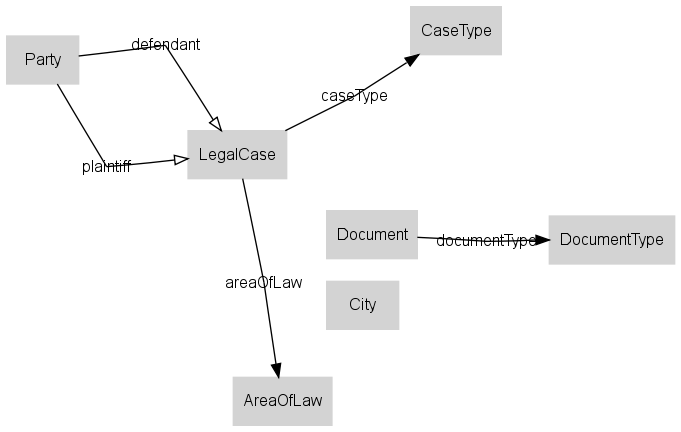
\includegraphics{PatCaseRegistration}}
\caption{Conceptual model of CaseRegistration}
\label{fig:PatCaseRegistration}
\end{center}
\end{figure}
\begin{description}
\item[rule@line70]
To arrive at the formalization in equation~\ref{DefRule:rule@line70}, the following four relations are introduced.
\begin{eqnarray}
   {\id{plaintiff}}&:&{\id{Party}}{\times}{\id{LegalCase}}\label{DefDecl:plaintiffPartyLegalCase}\\
   {\id{plaintiff}}&:&{\id{Party}}{\times}{\id{LegalCase}}\label{DefDecl:plaintiffPartyLegalCase}\\
   {\id{organization}}&:&{\id{Party}}{\times}{\id{Party}}\label{DefDecl:organizationPartyParty}\\
   {\id{person}}&:&{\id{Party}}{\times}{\id{Party}}\label{DefDecl:personPartyParty}
\end{eqnarray}

This means: 
\begin{equation}
   {\id{plaintiff}};{\id{plaintiff}}~{\cap}I_{[Party]}\ {\vdash}\ {\id{person}}{\cup}{\id{organization}}\label{DefRule:rule@line70}
\end{equation}

This corresponds to requirement~\ref{ReqRule:rule@line70} on page~\pageref{ReqRule:rule@line70}.
\item[rule@line73]
To arrive at the formalization in equation~\ref{DefRule:rule@line73}, the following three relations are introduced.
\begin{eqnarray}
   {\id{defendant}}&:&{\id{Party}}{\times}{\id{LegalCase}}\label{DefDecl:defendantPartyLegalCase}\\
   {\id{defendant}}&:&{\id{Party}}{\times}{\id{LegalCase}}\label{DefDecl:defendantPartyLegalCase}\\
   {\id{administrativeAuthority}}&:&{\id{Party}}{\times}{\id{Party}}\label{DefDecl:administrativeAuthorityPartyParty}
\end{eqnarray}

This means: 
\begin{equation}
   {\id{defendant}};{\id{defendant}}~{\cap}I_{[Party]}\ {\vdash}\ {\id{administrativeAuthority}}\label{DefRule:rule@line73}
\end{equation}

This corresponds to requirement~\ref{ReqRule:rule@line73} on page~\pageref{ReqRule:rule@line73}.
\item[rule@line84]
To arrive at the formalization in equation~\ref{DefRule:rule@line84}, the following two relations are introduced.
\begin{eqnarray}
   {\id{authFor}}&:&{\id{Document}}{\times}{\id{LegalCase}}\label{DefDecl:authForDocumentLegalCase}\\
   {\id{caseFile}}&:&{\id{Document}}{\times}{\id{LegalCase}}\label{DefDecl:caseFileDocumentLegalCase}
\end{eqnarray}

This means: 
\begin{equation}
   {\id{authFor}}{\cap}{\id{caseFile}}\ {\vdash}\ -V\label{DefRule:rule@line84}
\end{equation}

This corresponds to requirement~\ref{ReqRule:rule@line84} on page~\pageref{ReqRule:rule@line84}.
\item[rule@line92]
To arrive at the formalization in equation~\ref{DefRule:rule@line92}, the following three relations are introduced.
\begin{eqnarray}
   {\id{objection}}&:&{\id{LegalCase}}{\times}{\id{LegalCase}}\label{DefDecl:objectionLegalCaseLegalCase}\\
   {\id{appealToAdminCourt}}&:&{\id{LegalCase}}{\times}{\id{LegalCase}}\label{DefDecl:appealToAdminCourtLegalCaseLegalCase}\\
   {\id{appeal}}&:&{\id{LegalCase}}{\times}{\id{LegalCase}}\label{DefDecl:appealLegalCaseLegalCase}
\end{eqnarray}

This means: 
\begin{equation}
   I_{[LegalCase]}\ {\vdash}\ ({\id{appeal}}{\cup}{\id{appealToAdminCourt}}{\cup}{\id{objection}}){\cap}(\cmpl{{\id{appeal}}}{\cup}\cmpl{{\id{appealToAdminCourt}}}{\cup}\cmpl{{\id{objection}}})\label{DefRule:rule@line92}
\end{equation}

This corresponds to requirement~\ref{ReqRule:rule@line92} on page~\pageref{ReqRule:rule@line92}.
\item[rule@line103]
We use definitions \ref{DefDecl:administrativeAuthorityPartyParty} ({\id{administrativeAuthority}}), \ref{DefDecl:organizationPartyParty} ({\id{organization}}), and \ref{DefDecl:personPartyParty} ({\id{person}}). 
This means: 
\begin{equation}
   I_{[Party]}\ {\vdash}\ ({\id{person}}{\cup}{\id{organization}}{\cup}{\id{administrativeAuthority}}){\cap}(\cmpl{{\id{person}}}{\cup}\cmpl{{\id{organization}}}{\cup}\cmpl{{\id{administrativeAuthority}}})\label{DefRule:rule@line103}
\end{equation}

\item[rule@line107]
In order to formalize this, a relation
memberOfGovernment is introduced (\ref{DefDecl:memberOfGovernmentPartyParty}):
\begin{eqnarray}
   {\id{memberOfGovernment}}&:&{\id{Party}}{\times}{\id{Party}}\label{DefDecl:memberOfGovernmentPartyParty}
\end{eqnarray}

Beside that, we use definition \ref{DefDecl:administrativeAuthorityPartyParty}
(administrativeAuthority) to formalize requirement~\ref{ReqRule:rule@line107} (page~\pageref{ReqRule:rule@line107}):
This means: 
\begin{equation}
   {\id{memberOfGovernment}}\ {\vdash}\ {\id{administrativeAuthority}}\label{DefRule:rule@line107}
\end{equation}

\end{description}
\section{Sessions}

When administrative cases are brought before the district court, they
are assigned to a scheduled session with a certain panel of judges. The
registration of sessions is based on article 8:10 Awb.

Article 8:10 Awb

\begin{enumerate}[1.]
\item
  Cases brought before the district court shall first be considered by a
  single-judge panel.
\item
  If the single-judge panel deems a case unsuitable for consideration by
  a single judge, it will refer it to a three-judge panel. A
  single-judge panel may also refer a case to a three-judge panel for
  other reasons.
\item
  If a three-judge panel thinks that a case is suitable for further
  consideration by a single judge, it may refer it to a single-judge
  panel.
\item
  A case may be referred at any stage of the proceedings. The case shall
  then be resumed at the point at which it was referred.
\end{enumerate}
The organization of panels is defined in the Dutch law for the
administration of justice, 'Wet op de rechterlijke organisatie (RO)'.
For example article 6:1 RO describes that there are single-judge and
three-judge panels, of which the members are recognized judges. Article
41 par.1 RO defines that the district court is seated in the main city
of the jurisdiction. Article 41 par.2 RO allows for local offices of the
district court.

For illustration purposes, article 8:7 par.1 Awb will be maintained
within the 'VIRO' context.

Figure \ref{fig:PatSessions} shows a conceptual diagram of this theme.

\begin{figure}[htb]
\begin{center}
\scalebox{.3}[.3]{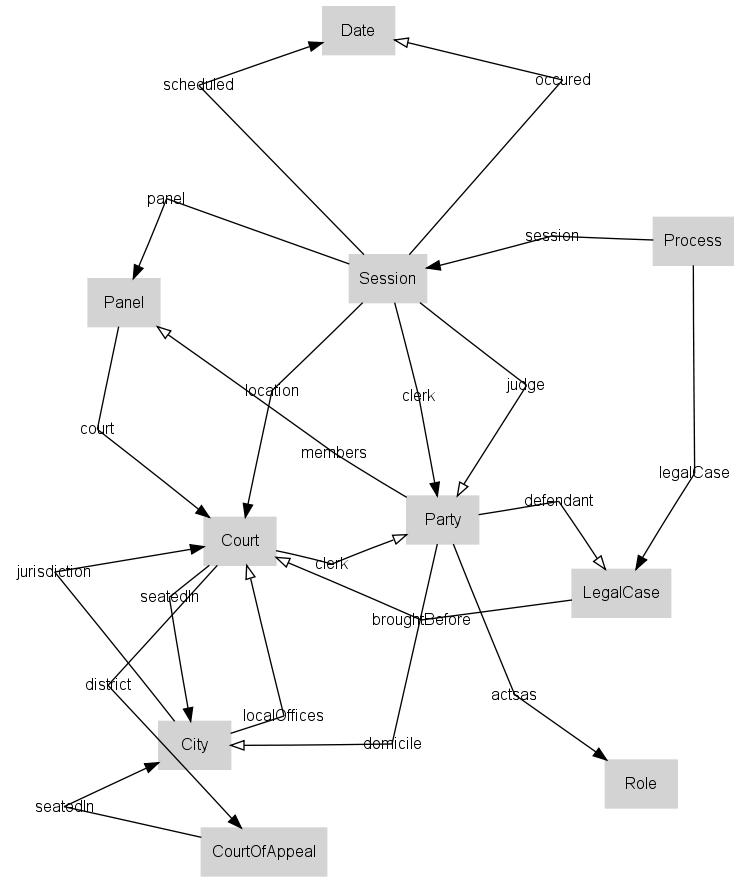
\includegraphics{PatSessions}}
\caption{Conceptual model of Sessions}
\label{fig:PatSessions}
\end{center}
\end{figure}
\begin{description}
\item[rule@line123]
To arrive at the formalization in equation~\ref{DefRule:rule@line123}, the following six relations are introduced.
\begin{eqnarray}
   {\id{scheduled}}&:&{\id{Session}}{\rightarrow}{\id{Date}}\label{DefDecl:scheduledSessionDate}\\
   {\id{scheduled}}&:&{\id{Session}}{\rightarrow}{\id{Date}}\label{DefDecl:scheduledSessionDate}\\
   {\id{location}}&:&{\id{Session}}{\rightarrow}{\id{Court}}\label{DefDecl:locationSessionCourt}\\
   {\id{location}}&:&{\id{Session}}{\rightarrow}{\id{Court}}\label{DefDecl:locationSessionCourt}\\
   {\id{panel}}&:&{\id{Session}}{\rightarrow}{\id{Panel}}\label{DefDecl:panelSessionPanel}\\
   {\id{panel}}&:&{\id{Session}}{\rightarrow}{\id{Panel}}\label{DefDecl:panelSessionPanel}
\end{eqnarray}

This means: 
\begin{equation}
   {\id{panel}};{\id{panel}}~{\cap}{\id{location}};{\id{location}}~{\cap}{\id{scheduled}};{\id{scheduled}}~\ {\vdash}\ I_{[Session]}\label{DefRule:rule@line123}
\end{equation}

This corresponds to requirement~\ref{ReqRule:rule@line123} on page~\pageref{ReqRule:rule@line123}.
\item[rule@line135]
To arrive at the formalization in equation~\ref{DefRule:rule@line135}, the following two relations are introduced.
\begin{eqnarray}
   {\id{judge}}&:&{\id{Session}}{\times}{\id{Party}}\label{DefDecl:judgeSessionParty}\\
   {\id{members}}&:&{\id{Party}}{\times}{\id{Panel}}\label{DefDecl:membersPartyPanel}
\end{eqnarray}

We also use definitions \ref{DefDecl:panelSessionPanel} ({\id{panel}}) and \ref{DefDecl:panelSessionPanel} ({\id{panel}}). 
This means: 
\begin{equation}
   {\id{judge}}\ {\vdash}\ {\id{panel}};{\id{members}}~\label{DefRule:rule@line135}
\end{equation}

This corresponds to requirement~\ref{ReqRule:rule@line135} on page~\pageref{ReqRule:rule@line135}.
\item[rule@line137]
To arrive at the formalization in equation~\ref{DefRule:rule@line137}, the following two relations are introduced.
\begin{eqnarray}
   {\id{clerk}}&:&{\id{Session}}{\rightarrow}{\id{Party}}\label{DefDecl:clerkSessionParty}\\
   {\id{clerk}}&:&{\id{Court}}{\times}{\id{Party}}\label{DefDecl:clerkCourtParty}
\end{eqnarray}

We also use definitions \ref{DefDecl:locationSessionCourt} ({\id{location}}) and \ref{DefDecl:locationSessionCourt} ({\id{location}}). 
This means: 
\begin{equation}
   {\id{clerk}}\ {\vdash}\ {\id{location}};{\id{clerk}}\label{DefRule:rule@line137}
\end{equation}

This corresponds to requirement~\ref{ReqRule:rule@line137} on page~\pageref{ReqRule:rule@line137}.
\item[rule@line143]
In order to formalize this, a relation
occured is introduced (\ref{DefDecl:occuredSessionDate}):
\begin{eqnarray}
   {\id{occured}}&:&{\id{Session}}{\times}{\id{Date}}\label{DefDecl:occuredSessionDate}
\end{eqnarray}

We also use definitions \ref{DefDecl:scheduledSessionDate} ({\id{scheduled}}) and \ref{DefDecl:scheduledSessionDate} ({\id{scheduled}}) to formalize requirement~\ref{ReqRule:rule@line143} (page~\pageref{ReqRule:rule@line143}):
This means: 
\begin{equation}
   {\id{occured}}\ {\vdash}\ {\id{scheduled}}\label{DefRule:rule@line143}
\end{equation}

\item[rule@line149]
In order to formalize this, a relation
administrativeAuthorityAwb87 is introduced (\ref{DefDecl:administrativeAuthorityAwb87PartyParty}):
\begin{eqnarray}
   {\id{administrativeAuthorityAwb87}}&:&{\id{Party}}{\times}{\id{Party}}\label{DefDecl:administrativeAuthorityAwb87PartyParty}
\end{eqnarray}

Beside that, we use definition \ref{DefDecl:administrativeAuthorityPartyParty}
(administrativeAuthority) to formalize requirement~\ref{ReqRule:rule@line149} (page~\pageref{ReqRule:rule@line149}):
This means: 
\begin{equation}
   {\id{administrativeAuthorityAwb87}}\ {\vdash}\ {\id{administrativeAuthority}}\label{DefRule:rule@line149}
\end{equation}

\item[rule@line151]
To arrive at the formalization in equation~\ref{DefRule:rule@line151}, the following three relations are introduced.
\begin{eqnarray}
   {\id{jurisdiction}}&:&{\id{City}}{\rightarrow}{\id{Court}}\label{DefDecl:jurisdictionCityCourt}\\
   {\id{domicile}}&:&{\id{Party}}{\times}{\id{City}}\label{DefDecl:domicilePartyCity}\\
   {\id{broughtBefore}}&:&{\id{LegalCase}}{\times}{\id{Court}}\label{DefDecl:broughtBeforeLegalCaseCourt}
\end{eqnarray}

We also use definitions \ref{DefDecl:administrativeAuthorityAwb87PartyParty} ({\id{administrativeAuthorityAwb87}}), \ref{DefDecl:appealLegalCaseLegalCase} ({\id{appeal}}), \ref{DefDecl:defendantPartyLegalCase} ({\id{defendant}}), and \ref{DefDecl:defendantPartyLegalCase} ({\id{defendant}}). 
This means: 
\begin{equation}
   {\id{appeal}};{\id{defendant}}~;{\id{administrativeAuthorityAwb87}};{\id{domicile}};{\id{jurisdiction}}\ {\vdash}\ {\id{broughtBefore}}\label{DefRule:rule@line151}
\end{equation}

This corresponds to requirement~\ref{ReqRule:rule@line151} on page~\pageref{ReqRule:rule@line151}.
\end{description}
\section{Correspondence}

Communication data of documents in case files may be registered.

Figure \ref{fig:PatCorrespondence} shows a conceptual diagram of this theme.

\begin{figure}[htb]
\begin{center}
\scalebox{.3}[.3]{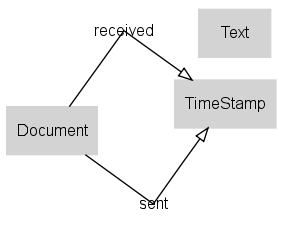
\includegraphics{PatCorrespondence}}
\caption{Conceptual model of Correspondence}
\label{fig:PatCorrespondence}
\end{center}
\end{figure}
\chapter{Process Analysis}\label{chpProcessAnalysis}

VIRO does not specify which roles may change the contents of which relations. 
VIRO assigns rules to roles. The following table shows the rules that are being maintained by a given role.

\begin{tabular}{|l|l|}\hline
Role&Rule\\ \hline
Archivist & file documents\\ \hline
   Scheduler & assign cases\\ \hline
\end{tabular}

\section{CaseFiles}

Figure \ref{fig:ProcCaseFiles} shows the process model.

\begin{figure}[htb]
\begin{center}
\scalebox{.3}[.3]{
\includegraphics{ProcCaseFiles}}
\caption{Process model of CaseFiles}
\label{fig:ProcCaseFiles}
\end{center}
\end{figure}
The conceptual diagram of figure \ref{fig:PLCaseFiles} provides an overview of the language in which this process is expressed.

\begin{figure}[htb]
\begin{center}
\scalebox{.3}[.3]{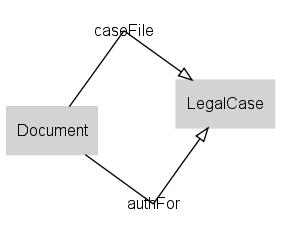
\includegraphics{PLCaseFiles}}
\caption{Basic sentences of CaseFiles}
\label{fig:PLCaseFiles}
\end{center}
\end{figure}
\begin{description}
\item[file documents]
We use definitions \ref{DefDecl:authForDocumentLegalCase} ({\id{authFor}}) and \ref{DefDecl:caseFileDocumentLegalCase} ({\id{caseFile}}). 
Activities that are defined by this rule are finished when: 
\begin{equation}
   I_{[Document]}\ {\vdash}\ {\id{caseFile}};{\id{caseFile}}~{\cup}{\id{authFor}};{\id{authFor}}~\label{DefRule:file documents}
\end{equation}

 These activities are signalled by:
\begin{equation}
   I_{[Document]}{\cap}\cmpl{({\id{caseFile}};{\id{caseFile}}~)}{\cap}\cmpl{({\id{authFor}};{\id{authFor}}~)}\label{DefRule:file documents}
\end{equation}

\end{description}
\section{Scheduling}

Figure \ref{fig:ProcScheduling} shows the process model.

\begin{figure}[htb]
\begin{center}
\scalebox{.3}[.3]{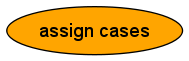
\includegraphics{ProcScheduling}}
\caption{Process model of Scheduling}
\label{fig:ProcScheduling}
\end{center}
\end{figure}
The conceptual diagram of figure \ref{fig:PLScheduling} provides an overview of the language in which this process is expressed.

\begin{figure}[htb]
\begin{center}
\scalebox{.3}[.3]{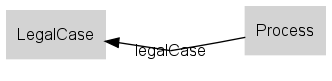
\includegraphics{PLScheduling}}
\caption{Basic sentences of Scheduling}
\label{fig:PLScheduling}
\end{center}
\end{figure}
\begin{description}
\item[assign cases]
We use definition \ref{DefDecl:legalCaseProcessLegalCase} (legalCase). 
Activities that are defined by this rule are finished when: 
\begin{equation}
   I_{[LegalCase]}\ {\vdash}\ {\id{legalCase}}~;{\id{legalCase}}\label{DefRule:assign cases}
\end{equation}

 These activities are signalled by:
\begin{equation}
   I_{[LegalCase]}{\cap}\cmpl{({\id{legalCase}}~;{\id{legalCase}})}\label{DefRule:assign cases}
\end{equation}

\end{description}
\chapter{Function Point Analysis}\label{chpFPAnalysis}

The specification of `VIRO' has been analysed by counting function points\cite{IFPUG}. This has resulted in an estimated total of 112 function points.

\begin{center}
\begin{tabular}{llr}
data set & analysis & FP\\
\hline
Party & ILGV Eenvoudig & 7\\
Session & ILGV Eenvoudig & 7\\
LegalCase & ILGV Eenvoudig & 7\\
Document & ILGV Eenvoudig & 7\\
Court & ILGV Eenvoudig & 7\\
Process & ILGV Eenvoudig & 7\\
City & ILGV Eenvoudig & 7\\
CourtOfAppeal & ILGV Eenvoudig & 7\\
Panel & ILGV Eenvoudig & 7\\
Text & ILGV Eenvoudig & 7\\
TimeStamp & ILGV Eenvoudig & 7\\
Date & ILGV Eenvoudig & 7\\
Role & ILGV Eenvoudig & 7\\
CaseType & ILGV Eenvoudig & 7\\
DocumentType & ILGV Eenvoudig & 7\\
AreaOfLaw & ILGV Eenvoudig & 7\\
\end{tabular}
\end{center}

\begin{center}
\begin{tabular}{llr}
interface & analysis & FP\\
\hline
file documents & NO & 0\\
assign cases & NO & 0\\
\end{tabular}
\end{center}

\chapter{Data structure}\label{chpDataAnalysis}

The requirements, which are listed in chapter \ref{chpFunctionalRequirements}, have been translated into the data model in figure \ref{fig:CDVIRO}. There are 9 data sets, 12 associations, no generalisations, and no aggregations. VIRO has a total of 16 concepts.

\begin{figure}[htb]
\begin{center}
\scalebox{.3}[.3]{
\includegraphics{CDclassificationVIRO}}
\caption{Classification of VIRO}
\label{fig:CDclassificationVIRO}
\end{center}
\end{figure}
\begin{figure}[htb]
\begin{center}
\scalebox{.3}[.3]{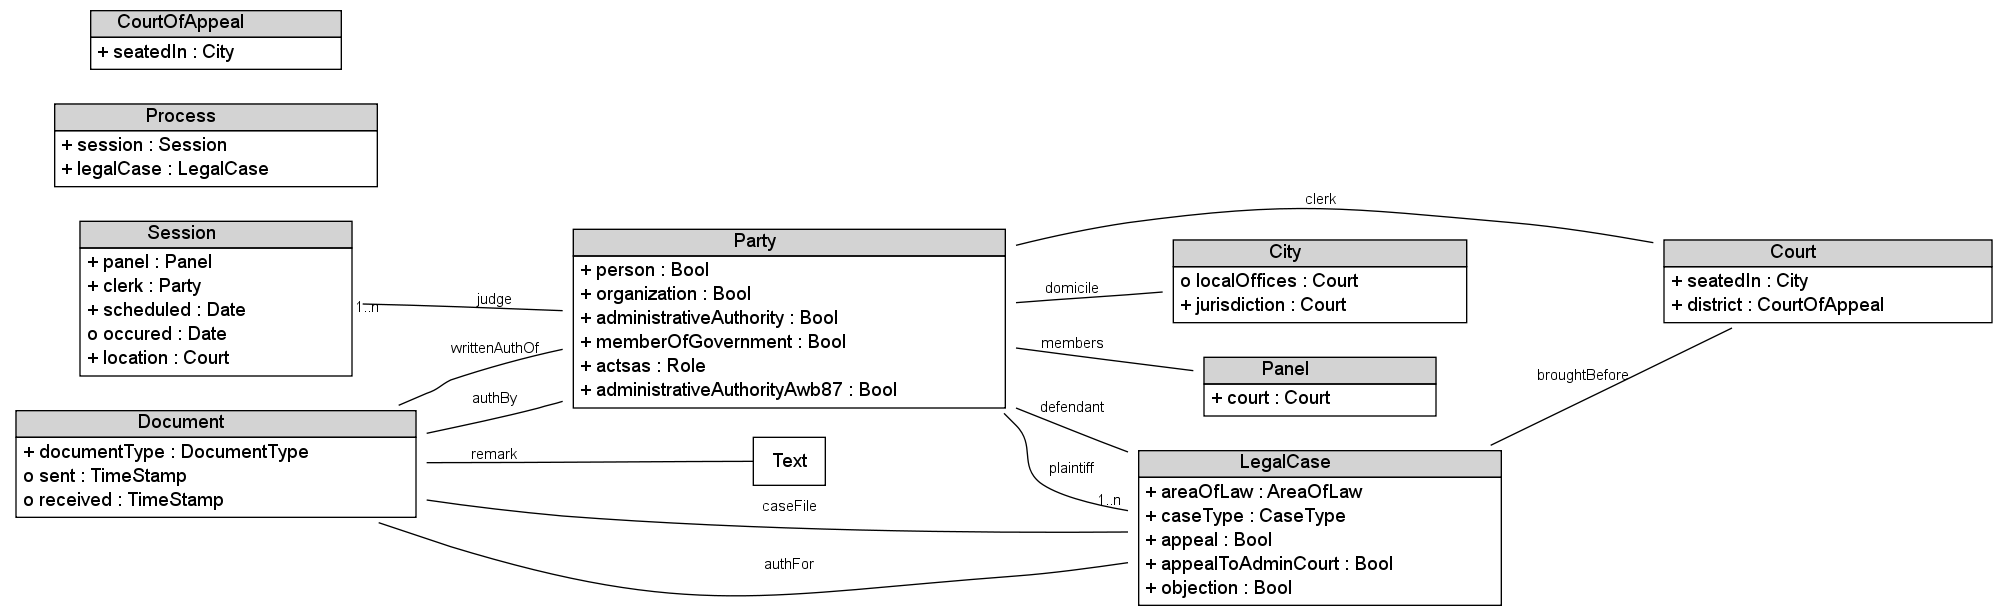
\includegraphics{CDVIRO}}
\caption{Data model of VIRO}
\label{fig:CDVIRO}
\end{center}
\end{figure}
VIRO has the following associations and multiplicity constraints. 

\begin{center}
\begin{tabular}{lcc}
relation & total & surjective\\
\hline
${\id{plaintiff}}$ &  & $\surd$\\
${\id{judge}}~$ &  & $\surd$\\
\end{tabular}
\end{center}

$Additionally, the endorelations come with the following properties: $

\begin{center}
\begin{tabular}{lcccccc}
relation & Rfx & Irf & Trn & Sym & Asy & Prop\\
\hline
${\id{objection}}$ &  &  &  & $\surd$ & $\surd$ & $\surd$\\
${\id{appealToAdminCourt}}$ &  &  &  & $\surd$ & $\surd$ & $\surd$\\
${\id{appeal}}$ &  &  &  & $\surd$ & $\surd$ & $\surd$\\
${\id{objection}}~$ &  &  &  & $\surd$ & $\surd$ & $\surd$\\
${\id{appealToAdminCourt}}~$ &  &  &  & $\surd$ & $\surd$ & $\surd$\\
${\id{appeal}}~$ &  &  &  & $\surd$ & $\surd$ & $\surd$\\
${\id{organization}}$ &  &  &  & $\surd$ & $\surd$ & $\surd$\\
${\id{person}}$ &  &  &  & $\surd$ & $\surd$ & $\surd$\\
${\id{administrativeAuthority}}$ &  &  &  & $\surd$ & $\surd$ & $\surd$\\
${\id{memberOfGovernment}}$ &  &  &  & $\surd$ & $\surd$ & $\surd$\\
${\id{administrativeAuthorityAwb87}}$ &  &  &  & $\surd$ & $\surd$ & $\surd$\\
\end{tabular}
\end{center}

\section{Party}

\label{sct:plug Party}

The attributes in Party have the following multiplicity constraints. 

\begin{center}
\begin{tabular}{llcc}
attribute & type & mandatory & unique\\
\hline
key  & Party & $\surd$ & $\surd$\\
person & Bool & $\surd$ & \\
organization & Bool & $\surd$ & \\
administrativeAuthority & Bool & $\surd$ & \\
memberOfGovernment & Bool & $\surd$ & \\
actsas & Role & $\surd$ & \\
administrativeAuthorityAwb87 & Bool & $\surd$ & \\
\end{tabular}
\end{center}

Within this data set, the following integrity rules shall be true at all times. 

\begin{itemize}
\item
  \[I_{[Party]}\ {\vdash}\ ({\id{person}}{\cup}{\id{organization}}{\cup}{\id{administrativeAuthority}}){\cap}\cmpl{({\id{person}}{\cap}{\id{organization}}{\cap}{\id{administrativeAuthority}})}\]
\item
  \[{\id{memberOfGovernment}}\ {\vdash}\ {\id{administrativeAuthority}}\]
\item
  \[{\id{administrativeAuthorityAwb87}}\ {\vdash}\ {\id{administrativeAuthority}}\]
\end{itemize}
The following rule defines the integrity of data within this data set. It must remain true at all times. 

\[\cmpl{I_{[Party]}}{\cup}({\id{person}}{\cup}{\id{organization}}{\cup}{\id{administrativeAuthority}}){\cap}(\cmpl{{\id{person}}}{\cup}\cmpl{{\id{organization}}}{\cup}\cmpl{{\id{administrativeAuthority}}})\]

\section{Session}

\label{sct:plug Session}

The attributes in Session have the following multiplicity constraints. 

\begin{center}
\begin{tabular}{llcc}
attribute & type & mandatory & unique\\
\hline
key  & Session & $\surd$ & $\surd$\\
panel & Panel & $\surd$ & \\
clerk & Party & $\surd$ & \\
scheduled & Date & $\surd$ & \\
occured & Date &  & \\
location & Court & $\surd$ & \\
\end{tabular}
\end{center}

Within this data set, the following integrity rule shall be true at all times. 

\[{\id{occured}}\ {\vdash}\ {\id{scheduled}}\]

\section{LegalCase}

\label{sct:plug LegalCase}

The attributes in LegalCase have the following multiplicity constraints. 

\begin{center}
\begin{tabular}{llcc}
attribute & type & mandatory & unique\\
\hline
key  & LegalCase & $\surd$ & $\surd$\\
areaOfLaw & AreaOfLaw & $\surd$ & \\
caseType & CaseType & $\surd$ & \\
appeal & Bool & $\surd$ & \\
appealToAdminCourt & Bool & $\surd$ & \\
objection & Bool & $\surd$ & \\
\end{tabular}
\end{center}

Within this data set, the following integrity rule shall be true at all times. 

\[I_{[LegalCase]}\ {\vdash}\ ({\id{appeal}}{\cup}{\id{appealToAdminCourt}}{\cup}{\id{objection}}){\cap}\cmpl{({\id{appeal}}{\cap}{\id{appealToAdminCourt}}{\cap}{\id{objection}})}\]

The following rules define the integrity of data within this data set. They must remain true at all times. 

\begin{itemize}
\item
  \[\cmpl{I_{[LegalCase]}}{\cup}({\id{appeal}}{\cup}{\id{appealToAdminCourt}}{\cup}{\id{objection}}){\cap}(\cmpl{{\id{appeal}}}{\cup}\cmpl{{\id{appealToAdminCourt}}}{\cup}\cmpl{{\id{objection}}})\]
\item
  \[\cmpl{I_{[LegalCase]}}{\cup}{\id{legalCase}}~;{\id{legalCase}}\]
\end{itemize}
\section{Document}

\label{sct:plug Document}

The attributes in Document have the following multiplicity constraints. 

\begin{center}
\begin{tabular}{llcc}
attribute & type & mandatory & unique\\
\hline
key  & Document & $\surd$ & $\surd$\\
documentType & DocumentType & $\surd$ & \\
sent & TimeStamp &  & \\
received & TimeStamp &  & \\
\end{tabular}
\end{center}

The following rule defines the integrity of data within this data set. It must remain true at all times. 

\[\cmpl{I_{[Document]}}{\cup}{\id{caseFile}};{\id{caseFile}}~{\cup}{\id{authFor}};{\id{authFor}}~\]

\section{Court}

\label{sct:plug Court}

The attributes in Court have the following multiplicity constraints. 

\begin{center}
\begin{tabular}{llcc}
attribute & type & mandatory & unique\\
\hline
key  & Court & $\surd$ & $\surd$\\
seatedIn & City & $\surd$ & \\
district & CourtOfAppeal & $\surd$ & \\
\end{tabular}
\end{center}

\section{Process}

\label{sct:plug Process}

The attributes in Process have the following multiplicity constraints. 

\begin{center}
\begin{tabular}{llcc}
attribute & type & mandatory & unique\\
\hline
key  & Process & $\surd$ & $\surd$\\
session & Session & $\surd$ & \\
legalCase & LegalCase & $\surd$ & \\
\end{tabular}
\end{center}

\section{City}

\label{sct:plug City}

The attributes in City have the following multiplicity constraints. 

\begin{center}
\begin{tabular}{llcc}
attribute & type & mandatory & unique\\
\hline
key  & City & $\surd$ & $\surd$\\
localOffices & Court &  & \\
jurisdiction & Court & $\surd$ & \\
\end{tabular}
\end{center}

\section{CourtOfAppeal}

\label{sct:plug CourtOfAppeal}

The attributes in CourtOfAppeal have the following multiplicity constraints. 

\begin{center}
\begin{tabular}{llcc}
attribute & type & mandatory & unique\\
\hline
key  & CourtOfAppeal & $\surd$ & $\surd$\\
seatedIn & City & $\surd$ & \\
\end{tabular}
\end{center}

\section{Panel}

\label{sct:plug Panel}

The attributes in Panel have the following multiplicity constraints. 

\begin{center}
\begin{tabular}{llcc}
attribute & type & mandatory & unique\\
\hline
key  & Panel & $\surd$ & $\surd$\\
court & Court & $\surd$ & \\
\end{tabular}
\end{center}

\section{plaintiff}

\label{sct:plug plaintiff}

The attributes in plaintiff have the following multiplicity constraints. 

\begin{center}
\begin{tabular}{llcc}
attribute & type & mandatory & unique\\
\hline
key  & LegalCase & $\surd$ & \\
Party & Party & $\surd$ & \\
\end{tabular}
\end{center}

The following rules define the integrity of data within this data set. They must remain true at all times. 

\begin{itemize}
\item
  \[\cmpl{I_{[LegalCase]}}{\cup}({\id{appeal}}{\cup}{\id{appealToAdminCourt}}{\cup}{\id{objection}}){\cap}(\cmpl{{\id{appeal}}}{\cup}\cmpl{{\id{appealToAdminCourt}}}{\cup}\cmpl{{\id{objection}}})\]
\item
  \[\cmpl{I_{[LegalCase]}}{\cup}{\id{legalCase}}~;{\id{legalCase}}\]
\end{itemize}
\section{defendant}

\label{sct:plug defendant}

The attributes in defendant have the following multiplicity constraints. 

\begin{center}
\begin{tabular}{llcc}
attribute & type & mandatory & unique\\
\hline
key  & Party & $\surd$ & \\
LegalCase & LegalCase & $\surd$ & \\
\end{tabular}
\end{center}

\section{domicile}

\label{sct:plug domicile}

The attributes in domicile have the following multiplicity constraints. 

\begin{center}
\begin{tabular}{llcc}
attribute & type & mandatory & unique\\
\hline
key  & Party & $\surd$ & \\
City & City & $\surd$ & \\
\end{tabular}
\end{center}

\section{writtenAuthOf}

\label{sct:plug writtenAuthOf}

The attributes in writtenAuthOf have the following multiplicity constraints. 

\begin{center}
\begin{tabular}{llcc}
attribute & type & mandatory & unique\\
\hline
key  & Document & $\surd$ & \\
Party & Party & $\surd$ & \\
\end{tabular}
\end{center}

\section{authFor}

\label{sct:plug authFor}

The attributes in authFor have the following multiplicity constraints. 

\begin{center}
\begin{tabular}{llcc}
attribute & type & mandatory & unique\\
\hline
key  & Document & $\surd$ & \\
LegalCase & LegalCase & $\surd$ & \\
\end{tabular}
\end{center}

\section{authBy}

\label{sct:plug authBy}

The attributes in authBy have the following multiplicity constraints. 

\begin{center}
\begin{tabular}{llcc}
attribute & type & mandatory & unique\\
\hline
key  & Document & $\surd$ & \\
Party & Party & $\surd$ & \\
\end{tabular}
\end{center}

\section{caseFile}

\label{sct:plug caseFile}

The attributes in caseFile have the following multiplicity constraints. 

\begin{center}
\begin{tabular}{llcc}
attribute & type & mandatory & unique\\
\hline
key  & Document & $\surd$ & \\
LegalCase & LegalCase & $\surd$ & \\
\end{tabular}
\end{center}

\section{members}

\label{sct:plug members}

The attributes in members have the following multiplicity constraints. 

\begin{center}
\begin{tabular}{llcc}
attribute & type & mandatory & unique\\
\hline
key  & Party & $\surd$ & \\
Panel & Panel & $\surd$ & \\
\end{tabular}
\end{center}

\section{judge}

\label{sct:plug judge}

The attributes in judge have the following multiplicity constraints. 

\begin{center}
\begin{tabular}{llcc}
attribute & type & mandatory & unique\\
\hline
key  & Session & $\surd$ & \\
Party & Party & $\surd$ & \\
\end{tabular}
\end{center}

\section{clerk}

\label{sct:plug clerk}

The attributes in clerk have the following multiplicity constraints. 

\begin{center}
\begin{tabular}{llcc}
attribute & type & mandatory & unique\\
\hline
key  & Court & $\surd$ & \\
Party & Party & $\surd$ & \\
\end{tabular}
\end{center}

\section{broughtBefore}

\label{sct:plug broughtBefore}

The attributes in broughtBefore have the following multiplicity constraints. 

\begin{center}
\begin{tabular}{llcc}
attribute & type & mandatory & unique\\
\hline
key  & LegalCase & $\surd$ & \\
Court & Court & $\surd$ & \\
\end{tabular}
\end{center}

\section{remark}

\label{sct:plug remark}

The attributes in remark have the following multiplicity constraints. 

\begin{center}
\begin{tabular}{llcc}
attribute & type & mandatory & unique\\
\hline
key  & Document & $\surd$ & \\
Text & Text & $\surd$ & \\
\end{tabular}
\end{center}

Figure \ref{fig:SBVIRO} shows the switchboard diagram.This is used in designing the database functionality.

\begin{figure}[htb]
\begin{center}
\scalebox{.3}[.3]{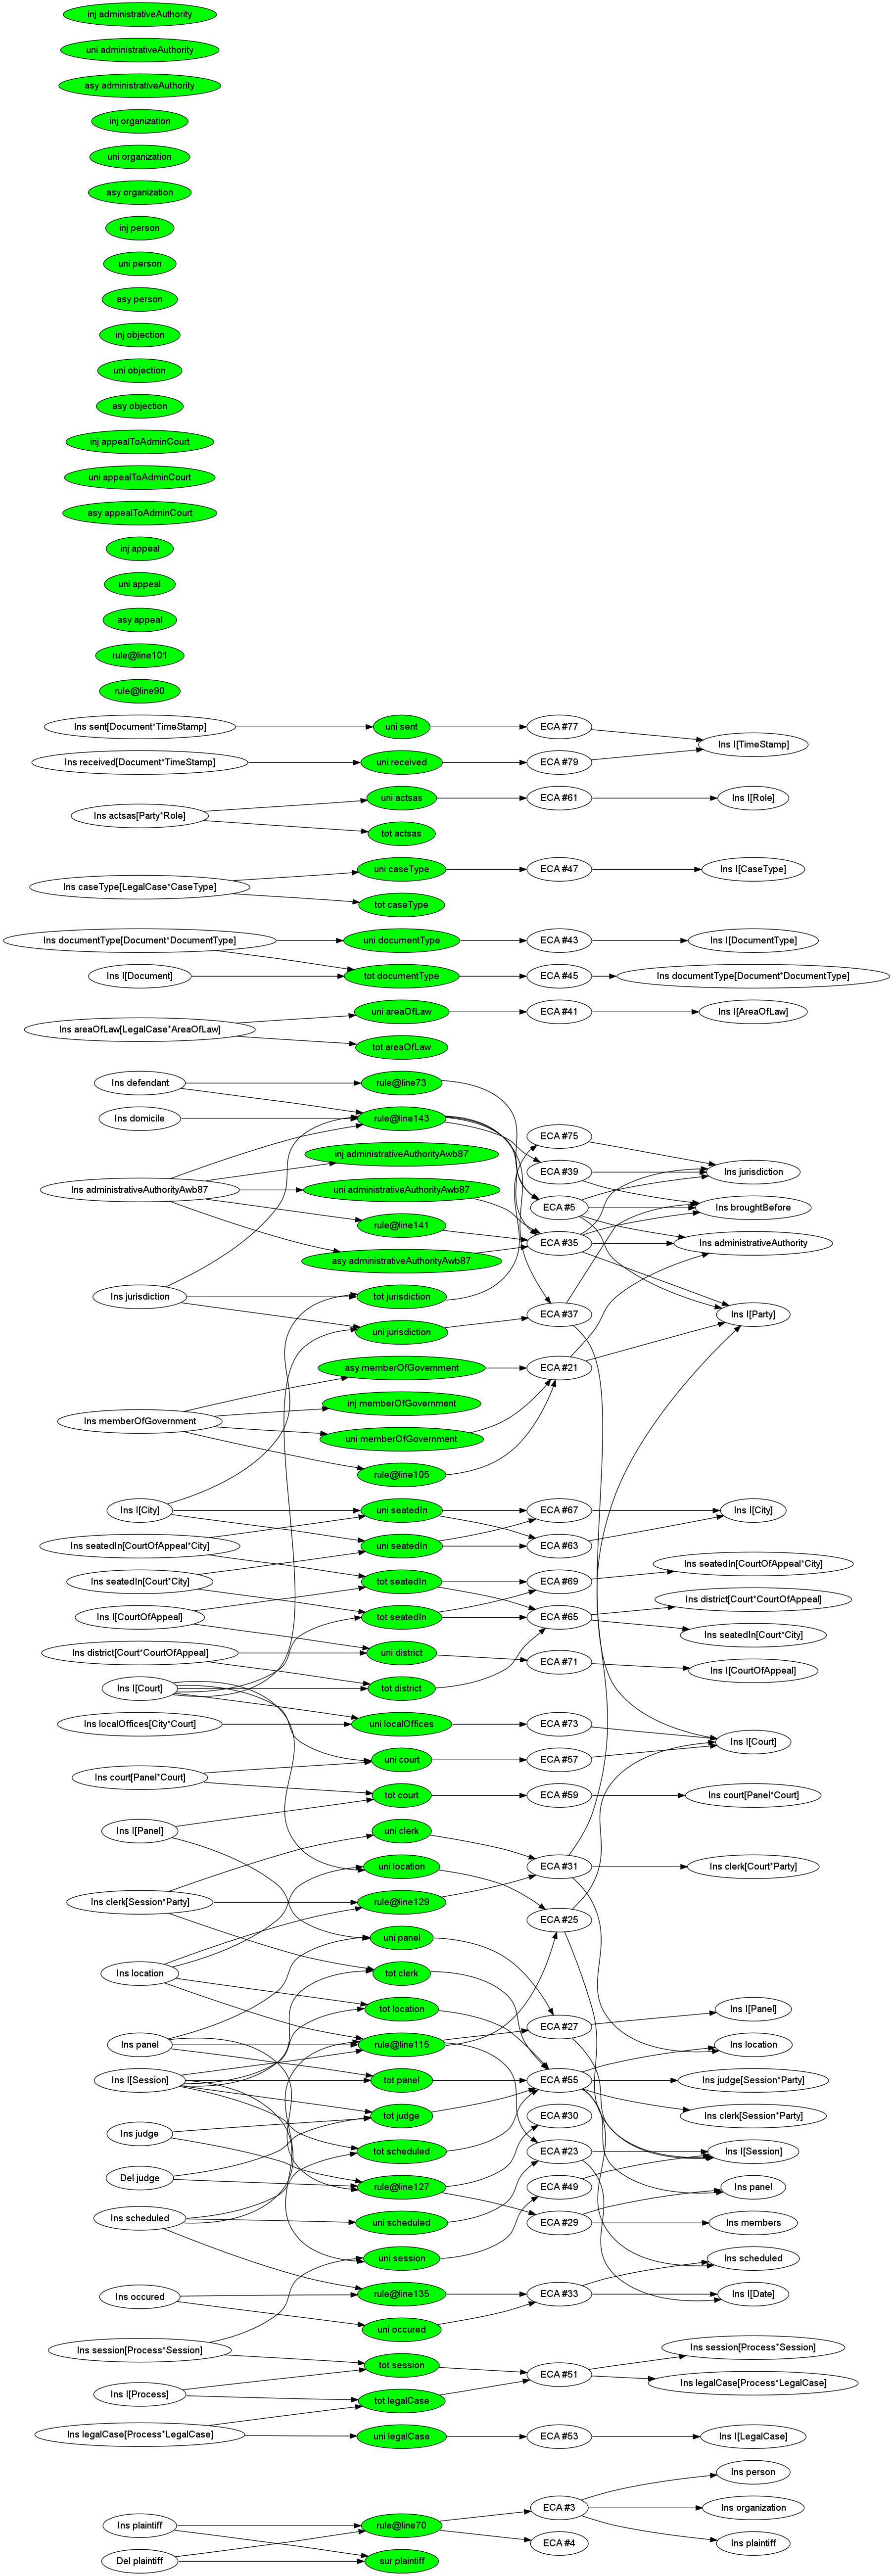
\includegraphics{SBVIRO}}
\caption{Switchboard of VIRO}
\label{fig:SBVIRO}
\end{center}
\end{figure}
\chapter{file documents}\label{chpIfcfile documents}

For what purpose activity `file documents' exists remains undocumented.
Activity `file documents'
must be performed by a user with role Archivist.
During that activity, rule `rule@line84'
will be maintained without intervention of a user.
The following table shows which edit actions invoke which function.
\begin{center}
\begin{tabular}{lll}
action & relation & rule\\
\hline
Ins & authFor{[}Document*LegalCase{]} & error: rule `rule@line84'\\
Del & authFor{[}Document*LegalCase{]} & error: rule `rule@line84'\\
Ins & caseFile{[}Document*LegalCase{]} & error: rule `rule@line84'\\
Del & caseFile{[}Document*LegalCase{]} & error: rule `rule@line84'\\
Ins & I & ECA rule 49\\
Del & I & error: rule `tot documentType'\\
\end{tabular}
\end{center}

Figure \ref{fig:Servfile_documents} shows the knowledge graph of this interface.

\begin{figure}[htb]
\begin{center}
\scalebox{.3}[.3]{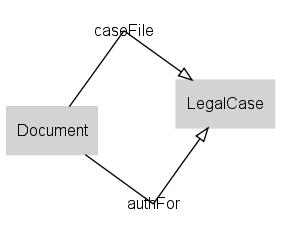
\includegraphics{Servfile_documents}}
\caption{Language diagram of file documents}
\label{fig:Servfile_documents}
\end{center}
\end{figure}
Every section in this chapter describes one activity. While performing an activity, users will insert or delete population in various relations. This may potentially violate invariants. (An invariant is a business rule rules that must remain true at all times.) The software to maintain the truth of invariant rules is generated automatically. The structure of that software is illustrated by a so called switchboard diagram, the first of which you will find in figure X. Each switchboard diagram consists of three columns: Invariant rules are drawn in the middle, and relations occur on the (right and left hand) sides. An arrow on the left hand side points from a relation that may be edited to a rule that may be violated as a consequence thereof. Each arrow on the right hand side of a rule represents an edit action that is required to restore its truth. It points to the relation that is edited for that purpose. If that arrow is labeled '+', it involves an insert event; if labeled '-' it refers to a delete event. This yields an accurate perspective on the way in which invariants are maintained. 

Figure \ref{fig:SBfile_documents} shows the switchboard diagram of this interface.

\begin{figure}[htb]
\begin{center}
\scalebox{.3}[.3]{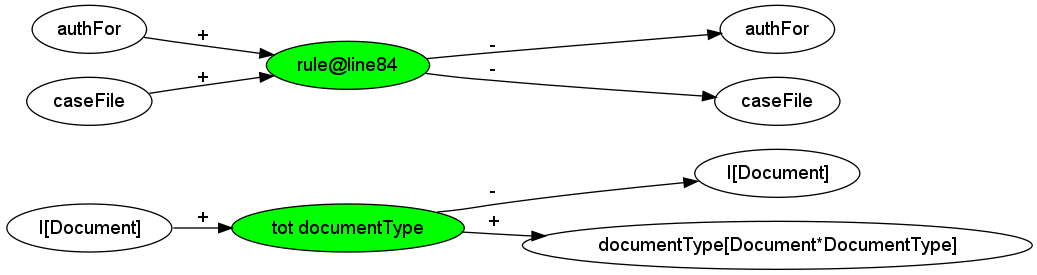
\includegraphics{SBfile_documents}}
\caption{Switchboard of file documents}
\label{fig:SBfile_documents}
\end{center}
\end{figure}
\chapter{assign cases}\label{chpIfcassign cases}

For what purpose activity `assign cases' exists remains undocumented.
Activity `assign cases' must be performed by a user with role Scheduler.
During that activity, rule `rule@line92'
will be maintained without intervention of a user.
The following table shows which edit actions invoke which function.
\begin{center}
\begin{tabular}{lll}
action & relation & rule\\
\hline
Ins & I & error: rule `asy appeal', `asy appealToAdminCourt', and `asy objection'\\
Del & I & error: rule `rule@line92', `sur plaintiff', `tot areaOfLaw', and `tot caseType'\\
Ins & legalCase{[}Process*LegalCase{]} & ECA rule 57\\
Del & legalCase{[}Process*LegalCase{]} & error: rule `uni legalCase'\\
\end{tabular}
\end{center}

Figure \ref{fig:Servassign_cases} shows the knowledge graph of this interface.

\begin{figure}[htb]
\begin{center}
\scalebox{.3}[.3]{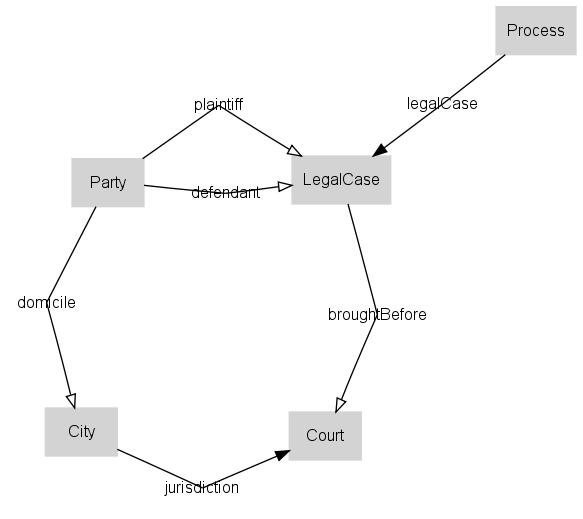
\includegraphics{Servassign_cases}}
\caption{Language diagram of assign cases}
\label{fig:Servassign_cases}
\end{center}
\end{figure}
Figure \ref{fig:SBassign_cases} shows the switchboard diagram of this interface.

\begin{figure}[htb]
\begin{center}
\scalebox{.3}[.3]{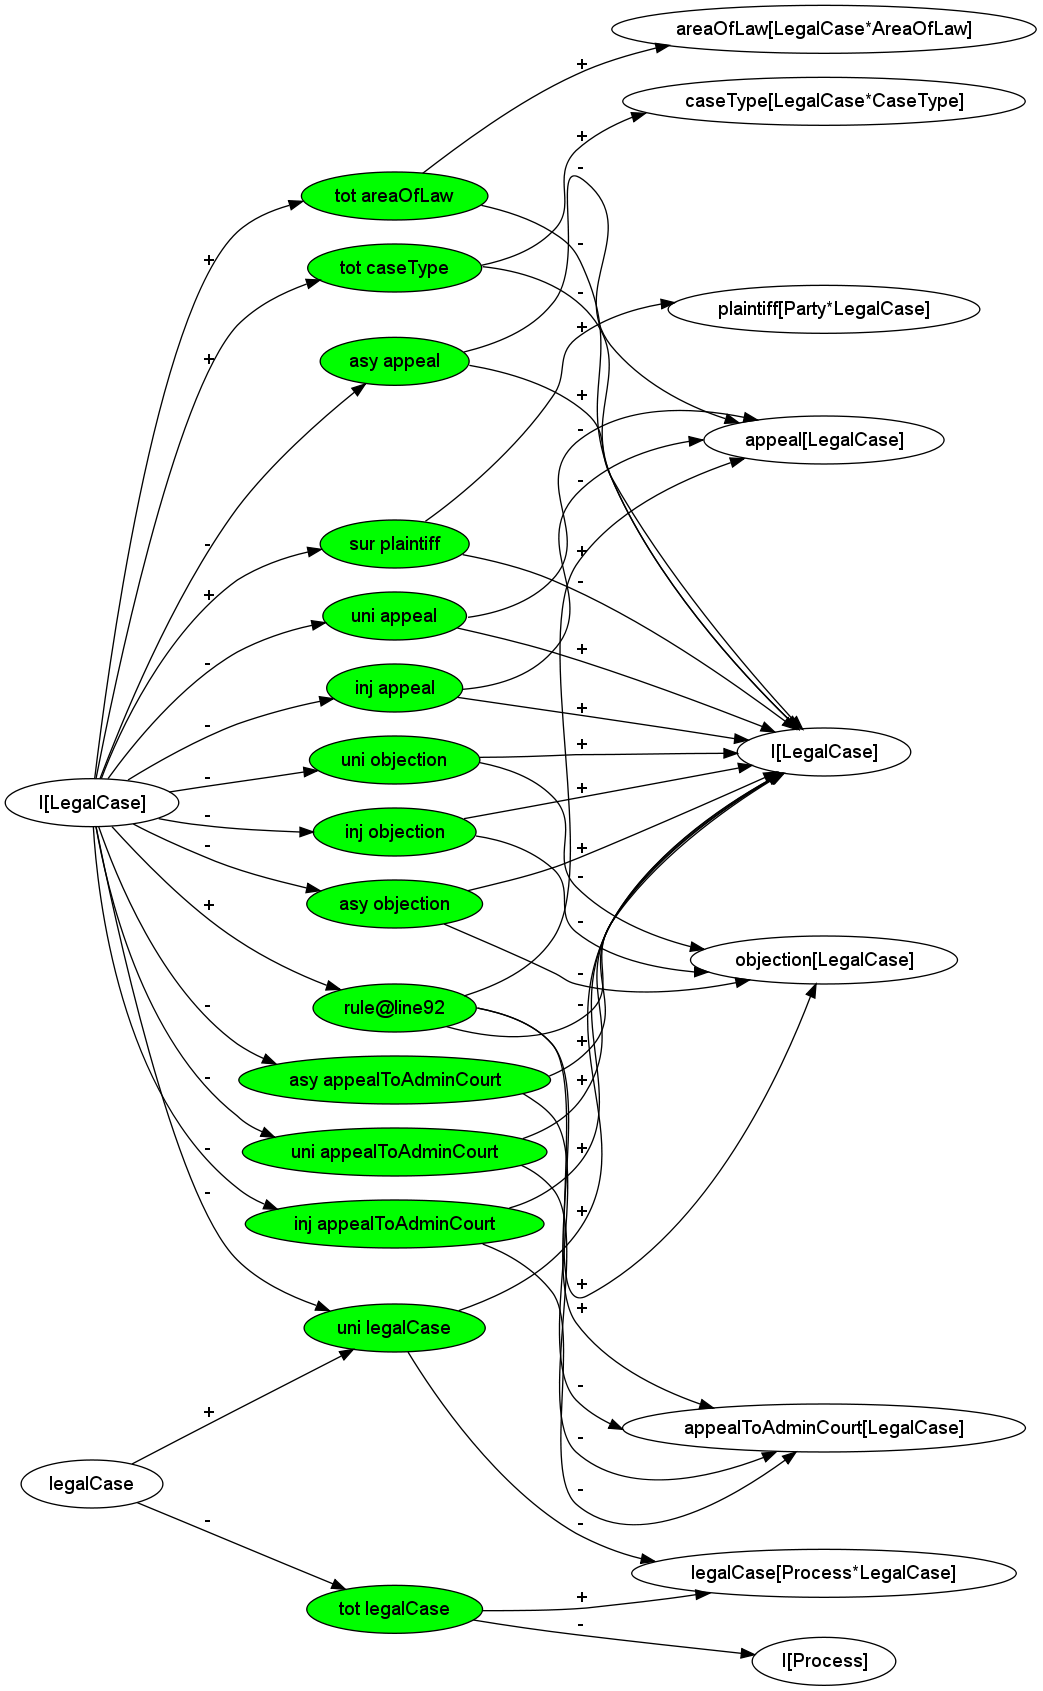
\includegraphics{SBassign_cases}}
\caption{Switchboard of assign cases}
\label{fig:SBassign_cases}
\end{center}
\end{figure}
\chapter{ECA rules}\label{chpECA}

This chapter lists the ECA rules.
ECA rules:\\   temporarily not documented

\begin{quote}
\begin{verbatim}
ON INSERT Delta IN I[Party] EXECUTE    -- (ECA rule 1)
BLOCK
(CANNOT CHANGE -(plaintiff;plaintiff~) \/ -I[Party] \/ person \/ organization FROM R3)
(CANNOT CHANGE -(defendant;defendant~) \/ -I[Party] \/ administrativeAuthority FROM R4)
(CANNOT CHANGE -person \/ -person \/ I[Party] FROM R0)
(CANNOT CHANGE -organization \/ -organization \/ I[Party] FROM R0)
(CANNOT CHANGE -administrativeAuthority \/ -administrativeAuthority \/ I[Party] FROM R0)
(CANNOT CHANGE -memberOfGovernment \/ -memberOfGovernment \/ I[Party] FROM R0)
(CANNOT CHANGE -administrativeAuthorityAwb87 \/ -administrativeAuthorityAwb87 \/ I[Party] FROM R0)
\end{verbatim}
\end{quote}
\begin{quote}
\begin{verbatim}
ON DELETE Delta FROM I[Party] EXECUTE    -- (ECA rule 2)
BLOCK
(CANNOT CHANGE -(plaintiff;plaintiff~) \/ -I[Party] \/ person \/ organization FROM R3)
(CANNOT CHANGE -I[Party] \/ (person \/ organization \/ administrativeAuthority)/\(-person \/ -organization \/ -administrativeAuthority) FROM R7)
(CANNOT CHANGE -I[Party] \/ actsas;actsas~ FROM R0)
\end{verbatim}
\end{quote}
\begin{quote}
\begin{verbatim}
ON INSERT Delta IN plaintiff EXECUTE    -- (ECA rule 3)
ONE of INSERT INTO person SELECTFROM
         (plaintiff;plaintiff~ \/ plaintiff;Delta~ \/ Delta;plaintiff~ \/ Delta;Delta~)/\-person/\-organization
       (TO MAINTAIN -(plaintiff;plaintiff~) \/ -I[Party] \/ person \/ organization FROM R3)
       INSERT INTO organization SELECTFROM
         (plaintiff;plaintiff~ \/ plaintiff;Delta~ \/ Delta;plaintiff~ \/ Delta;Delta~)/\-person/\-organization
       (TO MAINTAIN -(plaintiff;plaintiff~) \/ -I[Party] \/ person \/ organization FROM R3)
       CREATE x:Party;
         ALL of INSERT INTO person SELECTFROM
                  'x'[Party];V[Party*LegalCase];((plaintiff~ \/ Delta~)/\-(plaintiff~;person)/\-(Delta~;person)/\-(plaintiff~;organization)/\-(Delta~;organization)) \/ -(person)
                INSERT INTO plaintiff~ SELECTFROM
                  -(plaintiff~;person)/\-(Delta~;person)/\-(plaintiff~;organization)/\-(Delta~;organization) \/ Delta~/\-(plaintiff~;person)/\-(Delta~;person)/\-(plaintiff~;organization)/\-(Delta~;organization) \/ -plaintiff~
         (MAINTAINING -(plaintiff;plaintiff~) \/ -I[Party] \/ person \/ organization FROM R3)
       (MAINTAINING -(plaintiff;plaintiff~) \/ -I[Party] \/ person \/ organization FROM R3)
       SELECT x:Party FROM codomain(plaintiff~);
         INSERT INTO person SELECTFROM
           'x'[Party];V[Party*LegalCase];((plaintiff~ \/ Delta~)/\-(plaintiff~;person)/\-(Delta~;person)/\-(plaintiff~;organization)/\-(Delta~;organization)) \/ -(person)
       (MAINTAINING -(plaintiff;plaintiff~) \/ -I[Party] \/ person \/ organization FROM R3)
       SELECT x:Party FROM codomain(person~);
         INSERT INTO plaintiff~ SELECTFROM
           -(plaintiff~;person)/\-(Delta~;person)/\-(plaintiff~;organization)/\-(Delta~;organization) \/ Delta~/\-(plaintiff~;person)/\-(Delta~;person)/\-(plaintiff~;organization)/\-(Delta~;organization) \/ -plaintiff~
       (MAINTAINING -(plaintiff;plaintiff~) \/ -I[Party] \/ person \/ organization FROM R3)
       SELECT x:Party FROM codomain(plaintiff~);
         INSERT INTO organization SELECTFROM
           'x'[Party];V[Party*LegalCase];((plaintiff~ \/ Delta~)/\-(plaintiff~;person)/\-(Delta~;person)/\-(plaintiff~;organization)/\-(Delta~;organization)) \/ -(organization)
       (MAINTAINING -(plaintiff;plaintiff~) \/ -I[Party] \/ person \/ organization FROM R3)
       SELECT x:Party FROM codomain(organization~);
         INSERT INTO plaintiff~ SELECTFROM
           -(plaintiff~;person)/\-(Delta~;person)/\-(plaintiff~;organization)/\-(Delta~;organization) \/ Delta~/\-(plaintiff~;person)/\-(Delta~;person)/\-(plaintiff~;organization)/\-(Delta~;organization) \/ -plaintiff~
       (MAINTAINING -(plaintiff;plaintiff~) \/ -I[Party] \/ person \/ organization FROM R3)
       SELECT x:Party FROM codomain(person);
         INSERT INTO plaintiff SELECTFROM
           -(person;plaintiff)/\-(person;Delta)/\-(organization;plaintiff)/\-(organization;Delta) \/ Delta/\-(person;plaintiff)/\-(person;Delta)/\-(organization;plaintiff)/\-(organization;Delta) \/ -plaintiff
       (MAINTAINING -(plaintiff;plaintiff~) \/ -I[Party] \/ person \/ organization FROM R3)
       SELECT x:Party FROM codomain(plaintiff~);
         INSERT INTO person SELECTFROM
           ((plaintiff \/ Delta)/\-(person;plaintiff)/\-(person;Delta)/\-(organization;plaintiff)/\-(organization;Delta));V[LegalCase*Party];'x'[Party] \/ -(person)
       (MAINTAINING -(plaintiff;plaintiff~) \/ -I[Party] \/ person \/ organization FROM R3)
       SELECT x:Party FROM codomain(organization);
         INSERT INTO plaintiff SELECTFROM
           -(person;plaintiff)/\-(person;Delta)/\-(organization;plaintiff)/\-(organization;Delta) \/ Delta/\-(person;plaintiff)/\-(person;Delta)/\-(organization;plaintiff)/\-(organization;Delta) \/ -plaintiff
       (MAINTAINING -(plaintiff;plaintiff~) \/ -I[Party] \/ person \/ organization FROM R3)
       SELECT x:Party FROM codomain(plaintiff~);
         INSERT INTO organization SELECTFROM
           ((plaintiff \/ Delta)/\-(person;plaintiff)/\-(person;Delta)/\-(organization;plaintiff)/\-(organization;Delta));V[LegalCase*Party];'x'[Party] \/ -(organization)
       (MAINTAINING -(plaintiff;plaintiff~) \/ -I[Party] \/ person \/ organization FROM R3)
(MAINTAINING -(plaintiff;plaintiff~) \/ -I[Party] \/ person \/ organization FROM R3)
\end{verbatim}
\end{quote}
\begin{quote}
\begin{verbatim}
ON INSERT Delta IN defendant EXECUTE    -- (ECA rule 5)
ALL of ONE of INSERT INTO administrativeAuthority SELECTFROM
                (defendant;defendant~ \/ defendant;Delta~ \/ Delta;defendant~ \/ Delta;Delta~)/\(defendant;defendant~ \/ defendant;Delta~ \/ Delta;defendant~ \/ -administrativeAuthority)/\(defendant;defendant~ \/ defendant;Delta~ \/ -administrativeAuthority \/ Delta;Delta~)/\(defendant;defendant~ \/ defendant;Delta~ \/ -administrativeAuthority \/ -administrativeAuthority)/\(defendant;defendant~ \/ -administrativeAuthority \/ Delta;defendant~ \/ Delta;Delta~)/\(defendant;defendant~ \/ -administrativeAuthority \/ Delta;defendant~ \/ -administrativeAuthority)/\(defendant;defendant~ \/ -administrativeAuthority \/ -administrativeAuthority \/ Delta;Delta~)/\(defendant;defendant~ \/ -administrativeAuthority \/ -administrativeAuthority \/ -administrativeAuthority)/\(-administrativeAuthority \/ defendant;Delta~ \/ Delta;defendant~ \/ Delta;Delta~)/\(-administrativeAuthority \/ defendant;Delta~ \/ Delta;defendant~ \/ -administrativeAuthority)/\(-administrativeAuthority \/ defendant;Delta~ \/ -administrativeAuthority \/ Delta;Delta~)/\(-administrativeAuthority \/ defendant;Delta~ \/ -administrativeAuthority \/ -administrativeAuthority)/\(-administrativeAuthority \/ -administrativeAuthority \/ Delta;defendant~ \/ Delta;Delta~)/\(-administrativeAuthority \/ -administrativeAuthority \/ Delta;defendant~ \/ -administrativeAuthority)/\(-administrativeAuthority \/ -administrativeAuthority \/ -administrativeAuthority \/ Delta;Delta~)/\(-administrativeAuthority \/ -administrativeAuthority \/ -administrativeAuthority \/ -administrativeAuthority)
              (TO MAINTAIN -(defendant;defendant~) \/ -I[Party] \/ administrativeAuthority FROM R4)
              INSERT INTO I[Party] SELECTFROM
                (administrativeAuthority;defendant;defendant~ \/ administrativeAuthority;Delta;defendant~ \/ administrativeAuthority;defendant;Delta~ \/ administrativeAuthority;Delta;Delta~)/\-I[Party]
              (TO MAINTAIN -(defendant;defendant~) \/ -I[Party] \/ administrativeAuthority FROM R4)
              INSERT INTO I[Party] SELECTFROM
                (defendant;defendant~;administrativeAuthority \/ defendant;Delta~;administrativeAuthority \/ Delta;defendant~;administrativeAuthority \/ Delta;Delta~;administrativeAuthority)/\(defendant;defendant~;administrativeAuthority \/ defendant;Delta~;administrativeAuthority \/ Delta;defendant~;administrativeAuthority \/ -I[Party])/\(defendant;defendant~;administrativeAuthority \/ defendant;Delta~;administrativeAuthority \/ -I[Party] \/ Delta;Delta~;administrativeAuthority)/\(defendant;defendant~;administrativeAuthority \/ defendant;Delta~;administrativeAuthority \/ -I[Party] \/ -I[Party])/\(defendant;defendant~;administrativeAuthority \/ -I[Party] \/ Delta;defendant~;administrativeAuthority \/ Delta;Delta~;administrativeAuthority)/\(defendant;defendant~;administrativeAuthority \/ -I[Party] \/ Delta;defendant~;administrativeAuthority \/ -I[Party])/\(defendant;defendant~;administrativeAuthority \/ -I[Party] \/ -I[Party] \/ Delta;Delta~;administrativeAuthority)/\(defendant;defendant~;administrativeAuthority \/ -I[Party] \/ -I[Party] \/ -I[Party])/\(-I[Party] \/ defendant;Delta~;administrativeAuthority \/ Delta;defendant~;administrativeAuthority \/ Delta;Delta~;administrativeAuthority)/\(-I[Party] \/ defendant;Delta~;administrativeAuthority \/ Delta;defendant~;administrativeAuthority \/ -I[Party])/\(-I[Party] \/ defendant;Delta~;administrativeAuthority \/ -I[Party] \/ Delta;Delta~;administrativeAuthority)/\(-I[Party] \/ defendant;Delta~;administrativeAuthority \/ -I[Party] \/ -I[Party])/\(-I[Party] \/ -I[Party] \/ Delta;defendant~;administrativeAuthority \/ Delta;Delta~;administrativeAuthority)/\(-I[Party] \/ -I[Party] \/ Delta;defendant~;administrativeAuthority \/ -I[Party])/\(-I[Party] \/ -I[Party] \/ -I[Party] \/ Delta;Delta~;administrativeAuthority)/\(-I[Party] \/ -I[Party] \/ -I[Party] \/ -I[Party])
              (TO MAINTAIN -(defendant;defendant~) \/ -I[Party] \/ administrativeAuthority FROM R4)
       (MAINTAINING -(defendant;defendant~) \/ -I[Party] \/ administrativeAuthority FROM R4)
       ONE of INSERT INTO broughtBefore SELECTFROM
                (appeal;defendant~;administrativeAuthorityAwb87;domicile;jurisdiction \/ appeal;Delta~;administrativeAuthorityAwb87;domicile;jurisdiction)/\(appeal;defendant~;administrativeAuthorityAwb87;domicile;jurisdiction \/ -broughtBefore)/\(-broughtBefore \/ appeal;Delta~;administrativeAuthorityAwb87;domicile;jurisdiction)/\(-broughtBefore \/ -broughtBefore)
              (TO MAINTAIN -(appeal;defendant~;administrativeAuthorityAwb87;domicile;jurisdiction) \/ broughtBefore FROM R14)
              CREATE x:Court;
                ALL of INSERT INTO jurisdiction~ SELECTFROM
                         V[Court*LegalCase];((appeal;defendant~;administrativeAuthorityAwb87;domicile \/ appeal;Delta~;administrativeAuthorityAwb87;domicile)/\-(broughtBefore;jurisdiction~)) \/ -jurisdiction~
                       INSERT INTO broughtBefore SELECTFROM
                         ((appeal;defendant~;administrativeAuthorityAwb87;domicile \/ appeal;Delta~;administrativeAuthorityAwb87;domicile)/\-(broughtBefore;jurisdiction~));V[City*Court] \/ -broughtBefore
                (MAINTAINING -(appeal;defendant~;administrativeAuthorityAwb87;domicile;jurisdiction) \/ broughtBefore FROM R14)
              (MAINTAINING -(appeal;defendant~;administrativeAuthorityAwb87;domicile;jurisdiction) \/ broughtBefore FROM R14)
              SELECT x:Court FROM codomain(broughtBefore);
                INSERT INTO jurisdiction~ SELECTFROM
                  V[Court*LegalCase];((appeal;defendant~;administrativeAuthorityAwb87;domicile \/ appeal;Delta~;administrativeAuthorityAwb87;domicile)/\-(broughtBefore;jurisdiction~)) \/ -jurisdiction~
              (MAINTAINING -(appeal;defendant~;administrativeAuthorityAwb87;domicile;jurisdiction) \/ broughtBefore FROM R14)
              SELECT x:Court FROM codomain(jurisdiction);
                INSERT INTO broughtBefore SELECTFROM
                  ((appeal;defendant~;administrativeAuthorityAwb87;domicile \/ appeal;Delta~;administrativeAuthorityAwb87;domicile)/\-(broughtBefore;jurisdiction~));V[City*Court] \/ -broughtBefore
              (MAINTAINING -(appeal;defendant~;administrativeAuthorityAwb87;domicile;jurisdiction) \/ broughtBefore FROM R14)
       (MAINTAINING -(appeal;defendant~;administrativeAuthorityAwb87;domicile;jurisdiction) \/ broughtBefore FROM R14)
(MAINTAINING -(defendant;defendant~) \/ -I[Party] \/ administrativeAuthority FROM R4)
(MAINTAINING -(appeal;defendant~;administrativeAuthorityAwb87;domicile;jurisdiction) \/ broughtBefore FROM R14)
\end{verbatim}
\end{quote}
\begin{quote}
\begin{verbatim}
ON DELETE Delta FROM defendant EXECUTE    -- (ECA rule 6)
BLOCK
(CANNOT CHANGE -(defendant;defendant~) \/ -I[Party] \/ administrativeAuthority FROM R4)
(CANNOT CHANGE -(appeal;defendant~;administrativeAuthorityAwb87;domicile;jurisdiction) \/ broughtBefore FROM R14)
\end{verbatim}
\end{quote}
\begin{quote}
\begin{verbatim}
ON INSERT Delta IN authFor EXECUTE    -- (ECA rule 7)
BLOCK
(CANNOT CHANGE -authFor \/ -caseFile FROM R5)
\end{verbatim}
\end{quote}
\begin{quote}
\begin{verbatim}
ON DELETE Delta FROM authFor EXECUTE    -- (ECA rule 8)
BLOCK
(CANNOT CHANGE -authFor \/ -caseFile FROM R5)
\end{verbatim}
\end{quote}
\begin{quote}
\begin{verbatim}
ON INSERT Delta IN caseFile EXECUTE    -- (ECA rule 9)
BLOCK
(CANNOT CHANGE -authFor \/ -caseFile FROM R5)
\end{verbatim}
\end{quote}
\begin{quote}
\begin{verbatim}
ON DELETE Delta FROM caseFile EXECUTE    -- (ECA rule 10)
BLOCK
(CANNOT CHANGE -authFor \/ -caseFile FROM R5)
\end{verbatim}
\end{quote}
\begin{quote}
\begin{verbatim}
ON INSERT Delta IN I[LegalCase] EXECUTE    -- (ECA rule 11)
BLOCK
(CANNOT CHANGE -appeal \/ -appeal \/ I[LegalCase] FROM R0)
(CANNOT CHANGE -appealToAdminCourt \/ -appealToAdminCourt \/ I[LegalCase] FROM R0)
(CANNOT CHANGE -objection \/ -objection \/ I[LegalCase] FROM R0)
\end{verbatim}
\end{quote}
\begin{quote}
\begin{verbatim}
ON DELETE Delta FROM I[LegalCase] EXECUTE    -- (ECA rule 12)
BLOCK
(CANNOT CHANGE -I[LegalCase] \/ (appeal \/ appealToAdminCourt \/ objection)/\(-appeal \/ -appealToAdminCourt \/ -objection) FROM R6)
(CANNOT CHANGE -I[LegalCase] \/ plaintiff~;plaintiff FROM R0)
(CANNOT CHANGE -I[LegalCase] \/ areaOfLaw;areaOfLaw~ FROM R0)
(CANNOT CHANGE -I[LegalCase] \/ caseType;caseType~ FROM R0)
\end{verbatim}
\end{quote}
\begin{quote}
\begin{verbatim}
ON INSERT Delta IN objection EXECUTE    -- (ECA rule 13)
BLOCK
(CANNOT CHANGE -I[LegalCase] \/ (appeal \/ appealToAdminCourt \/ objection)/\(-appeal \/ -appealToAdminCourt \/ -objection) FROM R6)
\end{verbatim}
\end{quote}
\begin{quote}
\begin{verbatim}
ON DELETE Delta FROM objection EXECUTE    -- (ECA rule 14)
BLOCK
(CANNOT CHANGE -objection \/ -objection \/ I[LegalCase] FROM R0)
(CANNOT CHANGE -(objection;objection) \/ I[LegalCase] FROM R0)
\end{verbatim}
\end{quote}
\begin{quote}
\begin{verbatim}
ON INSERT Delta IN appealToAdminCourt EXECUTE    -- (ECA rule 15)
BLOCK
(CANNOT CHANGE -I[LegalCase] \/ (appeal \/ appealToAdminCourt \/ objection)/\(-appeal \/ -appealToAdminCourt \/ -objection) FROM R6)
\end{verbatim}
\end{quote}
\begin{quote}
\begin{verbatim}
ON DELETE Delta FROM appealToAdminCourt EXECUTE    -- (ECA rule 16)
BLOCK
(CANNOT CHANGE -appealToAdminCourt \/ -appealToAdminCourt \/ I[LegalCase] FROM R0)
(CANNOT CHANGE -(appealToAdminCourt;appealToAdminCourt) \/ I[LegalCase] FROM R0)
\end{verbatim}
\end{quote}
\begin{quote}
\begin{verbatim}
ON INSERT Delta IN appeal EXECUTE    -- (ECA rule 17)
BLOCK
(CANNOT CHANGE -I[LegalCase] \/ (appeal \/ appealToAdminCourt \/ objection)/\(-appeal \/ -appealToAdminCourt \/ -objection) FROM R6)
\end{verbatim}
\end{quote}
\begin{quote}
\begin{verbatim}
ON DELETE Delta FROM appeal EXECUTE    -- (ECA rule 18)
BLOCK
(CANNOT CHANGE -(appeal;defendant~;administrativeAuthorityAwb87;domicile;jurisdiction) \/ broughtBefore FROM R14)
(CANNOT CHANGE -appeal \/ -appeal \/ I[LegalCase] FROM R0)
(CANNOT CHANGE -(appeal;appeal) \/ I[LegalCase] FROM R0)
\end{verbatim}
\end{quote}
\begin{quote}
\begin{verbatim}
ON INSERT Delta IN administrativeAuthority EXECUTE    -- (ECA rule 19)
BLOCK
(CANNOT CHANGE -I[Party] \/ (person \/ organization \/ administrativeAuthority)/\(-person \/ -organization \/ -administrativeAuthority) FROM R7)
\end{verbatim}
\end{quote}
\begin{quote}
\begin{verbatim}
ON DELETE Delta FROM administrativeAuthority EXECUTE    -- (ECA rule 20)
BLOCK
(CANNOT CHANGE -administrativeAuthority \/ -administrativeAuthority \/ I[Party] FROM R0)
(CANNOT CHANGE -(administrativeAuthority;administrativeAuthority) \/ I[Party] FROM R0)
\end{verbatim}
\end{quote}
\begin{quote}
\begin{verbatim}
ON INSERT Delta IN organization EXECUTE    -- (ECA rule 21)
BLOCK
(CANNOT CHANGE -I[Party] \/ (person \/ organization \/ administrativeAuthority)/\(-person \/ -organization \/ -administrativeAuthority) FROM R7)
\end{verbatim}
\end{quote}
\begin{quote}
\begin{verbatim}
ON DELETE Delta FROM organization EXECUTE    -- (ECA rule 22)
BLOCK
(CANNOT CHANGE -organization \/ -organization \/ I[Party] FROM R0)
(CANNOT CHANGE -(organization;organization) \/ I[Party] FROM R0)
\end{verbatim}
\end{quote}
\begin{quote}
\begin{verbatim}
ON INSERT Delta IN person EXECUTE    -- (ECA rule 23)
BLOCK
(CANNOT CHANGE -I[Party] \/ (person \/ organization \/ administrativeAuthority)/\(-person \/ -organization \/ -administrativeAuthority) FROM R7)
\end{verbatim}
\end{quote}
\begin{quote}
\begin{verbatim}
ON DELETE Delta FROM person EXECUTE    -- (ECA rule 24)
BLOCK
(CANNOT CHANGE -person \/ -person \/ I[Party] FROM R0)
(CANNOT CHANGE -(person;person) \/ I[Party] FROM R0)
\end{verbatim}
\end{quote}
\begin{quote}
\begin{verbatim}
ON INSERT Delta IN memberOfGovernment EXECUTE    -- (ECA rule 25)
ALL of INSERT INTO (memberOfGovernment \/ Delta)/\(memberOfGovernment \/ -I[Party])/\(-I[Party] \/ Delta)/\(-I[Party] \/ -I[Party]) \/ (memberOfGovernment;memberOfGovernment \/ memberOfGovernment;Delta \/ Delta;memberOfGovernment \/ Delta;Delta)/\(memberOfGovernment;memberOfGovernment \/ memberOfGovernment;Delta \/ Delta;memberOfGovernment \/ -I[Party])/\(memberOfGovernment;memberOfGovernment \/ memberOfGovernment;Delta \/ -I[Party] \/ Delta;Delta)/\(memberOfGovernment;memberOfGovernment \/ memberOfGovernment;Delta \/ -I[Party] \/ -I[Party])/\(memberOfGovernment;memberOfGovernment \/ -I[Party] \/ Delta;memberOfGovernment \/ Delta;Delta)/\(memberOfGovernment;memberOfGovernment \/ -I[Party] \/ Delta;memberOfGovernment \/ -I[Party])/\(memberOfGovernment;memberOfGovernment \/ -I[Party] \/ -I[Party] \/ Delta;Delta)/\(memberOfGovernment;memberOfGovernment \/ -I[Party] \/ -I[Party] \/ -I[Party])/\(-I[Party] \/ memberOfGovernment;Delta \/ Delta;memberOfGovernment \/ Delta;Delta)/\(-I[Party] \/ memberOfGovernment;Delta \/ Delta;memberOfGovernment \/ -I[Party])/\(-I[Party] \/ memberOfGovernment;Delta \/ -I[Party] \/ Delta;Delta)/\(-I[Party] \/ memberOfGovernment;Delta \/ -I[Party] \/ -I[Party])/\(-I[Party] \/ -I[Party] \/ Delta;memberOfGovernment \/ Delta;Delta)/\(-I[Party] \/ -I[Party] \/ Delta;memberOfGovernment \/ -I[Party])/\(-I[Party] \/ -I[Party] \/ -I[Party] \/ Delta;Delta)/\(-I[Party] \/ -I[Party] \/ -I[Party] \/ -I[Party]) SELECTFROM
         (memberOfGovernment \/ Delta)/\(memberOfGovernment \/ -I[Party])/\(-I[Party] \/ Delta)/\(-I[Party] \/ -I[Party])
       (TO MAINTAIN -memberOfGovernment \/ -memberOfGovernment \/ I[Party] FROM R0)
       (TO MAINTAIN -(memberOfGovernment;memberOfGovernment) \/ I[Party] FROM R0)
       ONE of INSERT INTO administrativeAuthority SELECTFROM
                (memberOfGovernment \/ Delta)/\(memberOfGovernment \/ -administrativeAuthority)/\(-administrativeAuthority \/ Delta)/\(-administrativeAuthority \/ -administrativeAuthority)
              (TO MAINTAIN -memberOfGovernment \/ administrativeAuthority FROM R8)
              INSERT INTO I[Party] SELECTFROM
                (administrativeAuthority;memberOfGovernment \/ administrativeAuthority;Delta)/\(administrativeAuthority;memberOfGovernment \/ -I[Party])/\(-I[Party] \/ administrativeAuthority;Delta)/\(-I[Party] \/ -I[Party])
              (TO MAINTAIN -memberOfGovernment \/ administrativeAuthority FROM R8)
              INSERT INTO I[Party] SELECTFROM
                (memberOfGovernment;administrativeAuthority \/ Delta;administrativeAuthority)/\(memberOfGovernment;administrativeAuthority \/ -I[Party])/\(-I[Party] \/ Delta;administrativeAuthority)/\(-I[Party] \/ -I[Party])
              (TO MAINTAIN -memberOfGovernment \/ administrativeAuthority FROM R8)
       (MAINTAINING -memberOfGovernment \/ administrativeAuthority FROM R8)
(MAINTAINING -memberOfGovernment \/ administrativeAuthority FROM R8)
(MAINTAINING -memberOfGovernment \/ -memberOfGovernment \/ I[Party] FROM R0)
(MAINTAINING -(memberOfGovernment;memberOfGovernment) \/ I[Party] FROM R0)
\end{verbatim}
\end{quote}
\begin{quote}
\begin{verbatim}
ON DELETE Delta FROM memberOfGovernment EXECUTE    -- (ECA rule 26)
BLOCK
(CANNOT CHANGE -memberOfGovernment \/ administrativeAuthority FROM R8)
(CANNOT CHANGE -memberOfGovernment \/ -memberOfGovernment \/ I[Party] FROM R0)
(CANNOT CHANGE -(memberOfGovernment;memberOfGovernment) \/ I[Party] FROM R0)
\end{verbatim}
\end{quote}
\begin{quote}
\begin{verbatim}
ON INSERT Delta IN scheduled EXECUTE    -- (ECA rule 27)
ALL of INSERT INTO I[Session] SELECTFROM
         panel;panel~/\location;location~/\(scheduled;scheduled~ \/ scheduled;Delta~ \/ Delta;scheduled~ \/ Delta;Delta~)/\-I[Session]
       (TO MAINTAIN -(panel;panel~) \/ -(location;location~) \/ -(scheduled;scheduled~) \/ I[Session] FROM R9)
       INSERT INTO I[Date] SELECTFROM
         (scheduled~;scheduled \/ scheduled~;Delta \/ Delta~;scheduled \/ Delta~;Delta)/\(scheduled~;scheduled \/ scheduled~;Delta \/ Delta~;scheduled \/ -I[Date])/\(scheduled~;scheduled \/ scheduled~;Delta \/ -I[Date] \/ Delta~;Delta)/\(scheduled~;scheduled \/ scheduled~;Delta \/ -I[Date] \/ -I[Date])/\(scheduled~;scheduled \/ -I[Date] \/ Delta~;scheduled \/ Delta~;Delta)/\(scheduled~;scheduled \/ -I[Date] \/ Delta~;scheduled \/ -I[Date])/\(scheduled~;scheduled \/ -I[Date] \/ -I[Date] \/ Delta~;Delta)/\(scheduled~;scheduled \/ -I[Date] \/ -I[Date] \/ -I[Date])/\(-I[Date] \/ scheduled~;Delta \/ Delta~;scheduled \/ Delta~;Delta)/\(-I[Date] \/ scheduled~;Delta \/ Delta~;scheduled \/ -I[Date])/\(-I[Date] \/ scheduled~;Delta \/ -I[Date] \/ Delta~;Delta)/\(-I[Date] \/ scheduled~;Delta \/ -I[Date] \/ -I[Date])/\(-I[Date] \/ -I[Date] \/ Delta~;scheduled \/ Delta~;Delta)/\(-I[Date] \/ -I[Date] \/ Delta~;scheduled \/ -I[Date])/\(-I[Date] \/ -I[Date] \/ -I[Date] \/ Delta~;Delta)/\(-I[Date] \/ -I[Date] \/ -I[Date] \/ -I[Date])
       (TO MAINTAIN -(scheduled~;scheduled) \/ I[Date] FROM R0)
(MAINTAINING -(panel;panel~) \/ -(location;location~) \/ -(scheduled;scheduled~) \/ I[Session] FROM R9)
(MAINTAINING -(scheduled~;scheduled) \/ I[Date] FROM R0)
\end{verbatim}
\end{quote}
\begin{quote}
\begin{verbatim}
ON DELETE Delta FROM scheduled EXECUTE    -- (ECA rule 28)
BLOCK
(CANNOT CHANGE -(panel;panel~) \/ -(location;location~) \/ -(scheduled;scheduled~) \/ I[Session] FROM R9)
(CANNOT CHANGE -(scheduled~;scheduled) \/ I[Date] FROM R0)
\end{verbatim}
\end{quote}
\begin{quote}
\begin{verbatim}
ON INSERT Delta IN location EXECUTE    -- (ECA rule 29)
ALL of INSERT INTO I[Session] SELECTFROM
         panel;panel~/\(location;location~ \/ location;Delta~ \/ Delta;location~ \/ Delta;Delta~)/\scheduled;scheduled~/\-I[Session]
       (TO MAINTAIN -(panel;panel~) \/ -(location;location~) \/ -(scheduled;scheduled~) \/ I[Session] FROM R9)
       INSERT INTO I[Court] SELECTFROM
         (location~;location \/ location~;Delta \/ Delta~;location \/ Delta~;Delta)/\(location~;location \/ location~;Delta \/ Delta~;location \/ -I[Court])/\(location~;location \/ location~;Delta \/ -I[Court] \/ Delta~;Delta)/\(location~;location \/ location~;Delta \/ -I[Court] \/ -I[Court])/\(location~;location \/ -I[Court] \/ Delta~;location \/ Delta~;Delta)/\(location~;location \/ -I[Court] \/ Delta~;location \/ -I[Court])/\(location~;location \/ -I[Court] \/ -I[Court] \/ Delta~;Delta)/\(location~;location \/ -I[Court] \/ -I[Court] \/ -I[Court])/\(-I[Court] \/ location~;Delta \/ Delta~;location \/ Delta~;Delta)/\(-I[Court] \/ location~;Delta \/ Delta~;location \/ -I[Court])/\(-I[Court] \/ location~;Delta \/ -I[Court] \/ Delta~;Delta)/\(-I[Court] \/ location~;Delta \/ -I[Court] \/ -I[Court])/\(-I[Court] \/ -I[Court] \/ Delta~;location \/ Delta~;Delta)/\(-I[Court] \/ -I[Court] \/ Delta~;location \/ -I[Court])/\(-I[Court] \/ -I[Court] \/ -I[Court] \/ Delta~;Delta)/\(-I[Court] \/ -I[Court] \/ -I[Court] \/ -I[Court])
       (TO MAINTAIN -(location~;location) \/ I[Court] FROM R0)
(MAINTAINING -(panel;panel~) \/ -(location;location~) \/ -(scheduled;scheduled~) \/ I[Session] FROM R9)
(MAINTAINING -(location~;location) \/ I[Court] FROM R0)
\end{verbatim}
\end{quote}
\begin{quote}
\begin{verbatim}
ON DELETE Delta FROM location EXECUTE    -- (ECA rule 30)
BLOCK
(CANNOT CHANGE -(panel;panel~) \/ -(location;location~) \/ -(scheduled;scheduled~) \/ I[Session] FROM R9)
(CANNOT CHANGE -(location~;location) \/ I[Court] FROM R0)
\end{verbatim}
\end{quote}
\begin{quote}
\begin{verbatim}
ON INSERT Delta IN panel EXECUTE    -- (ECA rule 31)
ALL of INSERT INTO I[Session] SELECTFROM
         (panel;panel~ \/ panel;Delta~ \/ Delta;panel~ \/ Delta;Delta~)/\location;location~/\scheduled;scheduled~/\-I[Session]
       (TO MAINTAIN -(panel;panel~) \/ -(location;location~) \/ -(scheduled;scheduled~) \/ I[Session] FROM R9)
       INSERT INTO I[Panel] SELECTFROM
         (panel~;panel \/ panel~;Delta \/ Delta~;panel \/ Delta~;Delta)/\(panel~;panel \/ panel~;Delta \/ Delta~;panel \/ -I[Panel])/\(panel~;panel \/ panel~;Delta \/ -I[Panel] \/ Delta~;Delta)/\(panel~;panel \/ panel~;Delta \/ -I[Panel] \/ -I[Panel])/\(panel~;panel \/ -I[Panel] \/ Delta~;panel \/ Delta~;Delta)/\(panel~;panel \/ -I[Panel] \/ Delta~;panel \/ -I[Panel])/\(panel~;panel \/ -I[Panel] \/ -I[Panel] \/ Delta~;Delta)/\(panel~;panel \/ -I[Panel] \/ -I[Panel] \/ -I[Panel])/\(-I[Panel] \/ panel~;Delta \/ Delta~;panel \/ Delta~;Delta)/\(-I[Panel] \/ panel~;Delta \/ Delta~;panel \/ -I[Panel])/\(-I[Panel] \/ panel~;Delta \/ -I[Panel] \/ Delta~;Delta)/\(-I[Panel] \/ panel~;Delta \/ -I[Panel] \/ -I[Panel])/\(-I[Panel] \/ -I[Panel] \/ Delta~;panel \/ Delta~;Delta)/\(-I[Panel] \/ -I[Panel] \/ Delta~;panel \/ -I[Panel])/\(-I[Panel] \/ -I[Panel] \/ -I[Panel] \/ Delta~;Delta)/\(-I[Panel] \/ -I[Panel] \/ -I[Panel] \/ -I[Panel])
       (TO MAINTAIN -(panel~;panel) \/ I[Panel] FROM R0)
(MAINTAINING -(panel;panel~) \/ -(location;location~) \/ -(scheduled;scheduled~) \/ I[Session] FROM R9)
(MAINTAINING -(panel~;panel) \/ I[Panel] FROM R0)
\end{verbatim}
\end{quote}
\begin{quote}
\begin{verbatim}
ON DELETE Delta FROM panel EXECUTE    -- (ECA rule 32)
BLOCK
(CANNOT CHANGE -(panel;panel~) \/ -(location;location~) \/ -(scheduled;scheduled~) \/ I[Session] FROM R9)
(CANNOT CHANGE -(panel~;panel) \/ I[Panel] FROM R0)
\end{verbatim}
\end{quote}
\begin{quote}
\begin{verbatim}
ON INSERT Delta IN judge EXECUTE    -- (ECA rule 33)
ONE of CREATE x:Panel;
         ALL of INSERT INTO members~ SELECTFROM
                  V[Panel*Session];((judge \/ Delta)/\-(panel;members~)) \/ -members~
                INSERT INTO panel SELECTFROM
                  ((judge \/ Delta)/\-(panel;members~));V[Party*Panel] \/ -panel
         (MAINTAINING -judge \/ panel;members~ FROM R10)
       (MAINTAINING -judge \/ panel;members~ FROM R10)
       SELECT x:Panel FROM codomain(panel);
         INSERT INTO members~ SELECTFROM
           V[Panel*Session];((judge \/ Delta)/\-(panel;members~)) \/ -members~
       (MAINTAINING -judge \/ panel;members~ FROM R10)
       SELECT x:Panel FROM codomain(members);
         INSERT INTO panel SELECTFROM
           ((judge \/ Delta)/\-(panel;members~));V[Party*Panel] \/ -panel
       (MAINTAINING -judge \/ panel;members~ FROM R10)
       INSERT INTO members~ SELECTFROM
         (panel~;judge \/ panel~;Delta)/\(panel~;judge \/ -members~)/\(-members~ \/ panel~;Delta)/\(-members~ \/ -members~)
       (TO MAINTAIN -judge \/ panel;members~ FROM R10)
(MAINTAINING -judge \/ panel;members~ FROM R10)
\end{verbatim}
\end{quote}
\begin{quote}
\begin{verbatim}
ON INSERT Delta IN clerk[Session*Party] EXECUTE    -- (ECA rule 35)
ALL of ONE of CREATE x:Court;
                ALL of INSERT INTO clerk[Court*Party] SELECTFROM
                         V[Court*Session];((clerk[Session*Party] \/ Delta)/\-(location;clerk[Court*Party])) \/ -clerk[Court*Party]
                       INSERT INTO location SELECTFROM
                         ((clerk[Session*Party] \/ Delta)/\-(location;clerk[Court*Party]));V[Party*Court] \/ -location
                (MAINTAINING -clerk[Session*Party] \/ location;clerk[Court*Party] FROM R11)
              (MAINTAINING -clerk[Session*Party] \/ location;clerk[Court*Party] FROM R11)
              SELECT x:Court FROM codomain(location);
                INSERT INTO clerk[Court*Party] SELECTFROM
                  V[Court*Session];((clerk[Session*Party] \/ Delta)/\-(location;clerk[Court*Party])) \/ -clerk[Court*Party]
              (MAINTAINING -clerk[Session*Party] \/ location;clerk[Court*Party] FROM R11)
              SELECT x:Court FROM codomain(clerk[Court*Party]~);
                INSERT INTO location SELECTFROM
                  ((clerk[Session*Party] \/ Delta)/\-(location;clerk[Court*Party]));V[Party*Court] \/ -location
              (MAINTAINING -clerk[Session*Party] \/ location;clerk[Court*Party] FROM R11)
              INSERT INTO clerk[Court*Party] SELECTFROM
                (location~;clerk[Session*Party] \/ location~;Delta)/\(location~;clerk[Session*Party] \/ -clerk[Court*Party])/\(-clerk[Court*Party] \/ location~;Delta)/\(-clerk[Court*Party] \/ -clerk[Court*Party])
              (TO MAINTAIN -clerk[Session*Party] \/ location;clerk[Court*Party] FROM R11)
       (MAINTAINING -clerk[Session*Party] \/ location;clerk[Court*Party] FROM R11)
       INSERT INTO I[Party] SELECTFROM
         (clerk[Session*Party]~;I[Session];clerk[Session*Party] \/ clerk[Session*Party]~;Delta \/ Delta~;clerk[Session*Party] \/ Delta~;Delta)/\(clerk[Session*Party]~;I[Session];clerk[Session*Party] \/ clerk[Session*Party]~;Delta \/ Delta~;clerk[Session*Party] \/ -I[Party])/\(clerk[Session*Party]~;I[Session];clerk[Session*Party] \/ clerk[Session*Party]~;Delta \/ -I[Party] \/ Delta~;Delta)/\(clerk[Session*Party]~;I[Session];clerk[Session*Party] \/ clerk[Session*Party]~;Delta \/ -I[Party] \/ -I[Party])/\(clerk[Session*Party]~;I[Session];clerk[Session*Party] \/ -I[Party] \/ Delta~;clerk[Session*Party] \/ Delta~;Delta)/\(clerk[Session*Party]~;I[Session];clerk[Session*Party] \/ -I[Party] \/ Delta~;clerk[Session*Party] \/ -I[Party])/\(clerk[Session*Party]~;I[Session];clerk[Session*Party] \/ -I[Party] \/ -I[Party] \/ Delta~;Delta)/\(clerk[Session*Party]~;I[Session];clerk[Session*Party] \/ -I[Party] \/ -I[Party] \/ -I[Party])/\(-I[Party] \/ clerk[Session*Party]~;Delta \/ Delta~;clerk[Session*Party] \/ Delta~;Delta)/\(-I[Party] \/ clerk[Session*Party]~;Delta \/ Delta~;clerk[Session*Party] \/ -I[Party])/\(-I[Party] \/ clerk[Session*Party]~;Delta \/ -I[Party] \/ Delta~;Delta)/\(-I[Party] \/ clerk[Session*Party]~;Delta \/ -I[Party] \/ -I[Party])/\(-I[Party] \/ -I[Party] \/ Delta~;clerk[Session*Party] \/ Delta~;Delta)/\(-I[Party] \/ -I[Party] \/ Delta~;clerk[Session*Party] \/ -I[Party])/\(-I[Party] \/ -I[Party] \/ -I[Party] \/ Delta~;Delta)/\(-I[Party] \/ -I[Party] \/ -I[Party] \/ -I[Party])
       (TO MAINTAIN -(clerk[Session*Party]~;I[Session];clerk[Session*Party]) \/ I[Party] FROM R0)
(MAINTAINING -clerk[Session*Party] \/ location;clerk[Court*Party] FROM R11)
(MAINTAINING -(clerk[Session*Party]~;I[Session];clerk[Session*Party]) \/ I[Party] FROM R0)
\end{verbatim}
\end{quote}
\begin{quote}
\begin{verbatim}
ON DELETE Delta FROM clerk[Session*Party] EXECUTE    -- (ECA rule 36)
BLOCK
(CANNOT CHANGE -(clerk[Session*Party]~;I[Session];clerk[Session*Party]) \/ I[Party] FROM R0)
\end{verbatim}
\end{quote}
\begin{quote}
\begin{verbatim}
ON INSERT Delta IN occured EXECUTE    -- (ECA rule 37)
ALL of ONE of INSERT INTO scheduled SELECTFROM
                (occured \/ Delta)/\(occured \/ -scheduled)/\(-scheduled \/ Delta)/\(-scheduled \/ -scheduled)
              (TO MAINTAIN -occured \/ scheduled FROM R12)
              INSERT INTO I[Date] SELECTFROM
                (scheduled~;occured \/ scheduled~;Delta)/\(scheduled~;occured \/ -I[Date])/\(-I[Date] \/ scheduled~;Delta)/\(-I[Date] \/ -I[Date])
              (TO MAINTAIN -occured \/ scheduled FROM R12)
       (MAINTAINING -occured \/ scheduled FROM R12)
       INSERT INTO I[Date] SELECTFROM
         (occured~;occured \/ occured~;Delta \/ Delta~;occured \/ Delta~;Delta)/\(occured~;occured \/ occured~;Delta \/ Delta~;occured \/ -I[Date])/\(occured~;occured \/ occured~;Delta \/ -I[Date] \/ Delta~;Delta)/\(occured~;occured \/ occured~;Delta \/ -I[Date] \/ -I[Date])/\(occured~;occured \/ -I[Date] \/ Delta~;occured \/ Delta~;Delta)/\(occured~;occured \/ -I[Date] \/ Delta~;occured \/ -I[Date])/\(occured~;occured \/ -I[Date] \/ -I[Date] \/ Delta~;Delta)/\(occured~;occured \/ -I[Date] \/ -I[Date] \/ -I[Date])/\(-I[Date] \/ occured~;Delta \/ Delta~;occured \/ Delta~;Delta)/\(-I[Date] \/ occured~;Delta \/ Delta~;occured \/ -I[Date])/\(-I[Date] \/ occured~;Delta \/ -I[Date] \/ Delta~;Delta)/\(-I[Date] \/ occured~;Delta \/ -I[Date] \/ -I[Date])/\(-I[Date] \/ -I[Date] \/ Delta~;occured \/ Delta~;Delta)/\(-I[Date] \/ -I[Date] \/ Delta~;occured \/ -I[Date])/\(-I[Date] \/ -I[Date] \/ -I[Date] \/ Delta~;Delta)/\(-I[Date] \/ -I[Date] \/ -I[Date] \/ -I[Date])
       (TO MAINTAIN -(occured~;occured) \/ I[Date] FROM R0)
(MAINTAINING -occured \/ scheduled FROM R12)
(MAINTAINING -(occured~;occured) \/ I[Date] FROM R0)
\end{verbatim}
\end{quote}
\begin{quote}
\begin{verbatim}
ON DELETE Delta FROM occured EXECUTE    -- (ECA rule 38)
BLOCK
(CANNOT CHANGE -occured \/ scheduled FROM R12)
(CANNOT CHANGE -(occured~;occured) \/ I[Date] FROM R0)
\end{verbatim}
\end{quote}
\begin{quote}
\begin{verbatim}
ON INSERT Delta IN administrativeAuthorityAwb87 EXECUTE    -- (ECA rule 39)
ALL of INSERT INTO (administrativeAuthorityAwb87 \/ Delta)/\(administrativeAuthorityAwb87 \/ -I[Party])/\(-I[Party] \/ Delta)/\(-I[Party] \/ -I[Party]) \/ (administrativeAuthorityAwb87;administrativeAuthorityAwb87 \/ administrativeAuthorityAwb87;Delta \/ Delta;administrativeAuthorityAwb87 \/ Delta;Delta)/\(administrativeAuthorityAwb87;administrativeAuthorityAwb87 \/ administrativeAuthorityAwb87;Delta \/ Delta;administrativeAuthorityAwb87 \/ -I[Party])/\(administrativeAuthorityAwb87;administrativeAuthorityAwb87 \/ administrativeAuthorityAwb87;Delta \/ -I[Party] \/ Delta;Delta)/\(administrativeAuthorityAwb87;administrativeAuthorityAwb87 \/ administrativeAuthorityAwb87;Delta \/ -I[Party] \/ -I[Party])/\(administrativeAuthorityAwb87;administrativeAuthorityAwb87 \/ -I[Party] \/ Delta;administrativeAuthorityAwb87 \/ Delta;Delta)/\(administrativeAuthorityAwb87;administrativeAuthorityAwb87 \/ -I[Party] \/ Delta;administrativeAuthorityAwb87 \/ -I[Party])/\(administrativeAuthorityAwb87;administrativeAuthorityAwb87 \/ -I[Party] \/ -I[Party] \/ Delta;Delta)/\(administrativeAuthorityAwb87;administrativeAuthorityAwb87 \/ -I[Party] \/ -I[Party] \/ -I[Party])/\(-I[Party] \/ administrativeAuthorityAwb87;Delta \/ Delta;administrativeAuthorityAwb87 \/ Delta;Delta)/\(-I[Party] \/ administrativeAuthorityAwb87;Delta \/ Delta;administrativeAuthorityAwb87 \/ -I[Party])/\(-I[Party] \/ administrativeAuthorityAwb87;Delta \/ -I[Party] \/ Delta;Delta)/\(-I[Party] \/ administrativeAuthorityAwb87;Delta \/ -I[Party] \/ -I[Party])/\(-I[Party] \/ -I[Party] \/ Delta;administrativeAuthorityAwb87 \/ Delta;Delta)/\(-I[Party] \/ -I[Party] \/ Delta;administrativeAuthorityAwb87 \/ -I[Party])/\(-I[Party] \/ -I[Party] \/ -I[Party] \/ Delta;Delta)/\(-I[Party] \/ -I[Party] \/ -I[Party] \/ -I[Party]) SELECTFROM
         (administrativeAuthorityAwb87 \/ Delta)/\(administrativeAuthorityAwb87 \/ -I[Party])/\(-I[Party] \/ Delta)/\(-I[Party] \/ -I[Party])
       (TO MAINTAIN -administrativeAuthorityAwb87 \/ -administrativeAuthorityAwb87 \/ I[Party] FROM R0)
       (TO MAINTAIN -(administrativeAuthorityAwb87;administrativeAuthorityAwb87) \/ I[Party] FROM R0)
       ONE of INSERT INTO administrativeAuthority SELECTFROM
                (administrativeAuthorityAwb87 \/ Delta)/\(administrativeAuthorityAwb87 \/ -administrativeAuthority)/\(-administrativeAuthority \/ Delta)/\(-administrativeAuthority \/ -administrativeAuthority)
              (TO MAINTAIN -administrativeAuthorityAwb87 \/ administrativeAuthority FROM R13)
              INSERT INTO I[Party] SELECTFROM
                (administrativeAuthority;administrativeAuthorityAwb87 \/ administrativeAuthority;Delta)/\(administrativeAuthority;administrativeAuthorityAwb87 \/ -I[Party])/\(-I[Party] \/ administrativeAuthority;Delta)/\(-I[Party] \/ -I[Party])
              (TO MAINTAIN -administrativeAuthorityAwb87 \/ administrativeAuthority FROM R13)
              INSERT INTO I[Party] SELECTFROM
                (administrativeAuthorityAwb87;administrativeAuthority \/ Delta;administrativeAuthority)/\(administrativeAuthorityAwb87;administrativeAuthority \/ -I[Party])/\(-I[Party] \/ Delta;administrativeAuthority)/\(-I[Party] \/ -I[Party])
              (TO MAINTAIN -administrativeAuthorityAwb87 \/ administrativeAuthority FROM R13)
       (MAINTAINING -administrativeAuthorityAwb87 \/ administrativeAuthority FROM R13)
       ONE of INSERT INTO broughtBefore SELECTFROM
                (appeal;defendant~;administrativeAuthorityAwb87;domicile;jurisdiction \/ appeal;defendant~;Delta;domicile;jurisdiction)/\(appeal;defendant~;administrativeAuthorityAwb87;domicile;jurisdiction \/ -broughtBefore)/\(-broughtBefore \/ appeal;defendant~;Delta;domicile;jurisdiction)/\(-broughtBefore \/ -broughtBefore)
              (TO MAINTAIN -(appeal;defendant~;administrativeAuthorityAwb87;domicile;jurisdiction) \/ broughtBefore FROM R14)
              CREATE x:Court;
                ALL of INSERT INTO jurisdiction~ SELECTFROM
                         V[Court*LegalCase];((appeal;defendant~;administrativeAuthorityAwb87;domicile \/ appeal;defendant~;Delta;domicile)/\-(broughtBefore;jurisdiction~)) \/ -jurisdiction~
                       INSERT INTO broughtBefore SELECTFROM
                         ((appeal;defendant~;administrativeAuthorityAwb87;domicile \/ appeal;defendant~;Delta;domicile)/\-(broughtBefore;jurisdiction~));V[City*Court] \/ -broughtBefore
                (MAINTAINING -(appeal;defendant~;administrativeAuthorityAwb87;domicile;jurisdiction) \/ broughtBefore FROM R14)
              (MAINTAINING -(appeal;defendant~;administrativeAuthorityAwb87;domicile;jurisdiction) \/ broughtBefore FROM R14)
              SELECT x:Court FROM codomain(broughtBefore);
                INSERT INTO jurisdiction~ SELECTFROM
                  V[Court*LegalCase];((appeal;defendant~;administrativeAuthorityAwb87;domicile \/ appeal;defendant~;Delta;domicile)/\-(broughtBefore;jurisdiction~)) \/ -jurisdiction~
              (MAINTAINING -(appeal;defendant~;administrativeAuthorityAwb87;domicile;jurisdiction) \/ broughtBefore FROM R14)
              SELECT x:Court FROM codomain(jurisdiction);
                INSERT INTO broughtBefore SELECTFROM
                  ((appeal;defendant~;administrativeAuthorityAwb87;domicile \/ appeal;defendant~;Delta;domicile)/\-(broughtBefore;jurisdiction~));V[City*Court] \/ -broughtBefore
              (MAINTAINING -(appeal;defendant~;administrativeAuthorityAwb87;domicile;jurisdiction) \/ broughtBefore FROM R14)
       (MAINTAINING -(appeal;defendant~;administrativeAuthorityAwb87;domicile;jurisdiction) \/ broughtBefore FROM R14)
(MAINTAINING -administrativeAuthorityAwb87 \/ administrativeAuthority FROM R13)
(MAINTAINING -(appeal;defendant~;administrativeAuthorityAwb87;domicile;jurisdiction) \/ broughtBefore FROM R14)
(MAINTAINING -administrativeAuthorityAwb87 \/ -administrativeAuthorityAwb87 \/ I[Party] FROM R0)
(MAINTAINING -(administrativeAuthorityAwb87;administrativeAuthorityAwb87) \/ I[Party] FROM R0)
\end{verbatim}
\end{quote}
\begin{quote}
\begin{verbatim}
ON DELETE Delta FROM administrativeAuthorityAwb87 EXECUTE    -- (ECA rule 40)
BLOCK
(CANNOT CHANGE -administrativeAuthorityAwb87 \/ administrativeAuthority FROM R13)
(CANNOT CHANGE -(appeal;defendant~;administrativeAuthorityAwb87;domicile;jurisdiction) \/ broughtBefore FROM R14)
(CANNOT CHANGE -administrativeAuthorityAwb87 \/ -administrativeAuthorityAwb87 \/ I[Party] FROM R0)
(CANNOT CHANGE -(administrativeAuthorityAwb87;administrativeAuthorityAwb87) \/ I[Party] FROM R0)
\end{verbatim}
\end{quote}
\begin{quote}
\begin{verbatim}
ON INSERT Delta IN jurisdiction EXECUTE    -- (ECA rule 41)
ALL of INSERT INTO broughtBefore SELECTFROM
         (appeal;defendant~;administrativeAuthorityAwb87;domicile;jurisdiction \/ appeal;defendant~;administrativeAuthorityAwb87;domicile;Delta)/\(appeal;defendant~;administrativeAuthorityAwb87;domicile;jurisdiction \/ -broughtBefore)/\(-broughtBefore \/ appeal;defendant~;administrativeAuthorityAwb87;domicile;Delta)/\(-broughtBefore \/ -broughtBefore)
       (TO MAINTAIN -(appeal;defendant~;administrativeAuthorityAwb87;domicile;jurisdiction) \/ broughtBefore FROM R14)
       INSERT INTO I[Court] SELECTFROM
         (jurisdiction~;jurisdiction \/ jurisdiction~;Delta \/ Delta~;jurisdiction \/ Delta~;Delta)/\(jurisdiction~;jurisdiction \/ jurisdiction~;Delta \/ Delta~;jurisdiction \/ -I[Court])/\(jurisdiction~;jurisdiction \/ jurisdiction~;Delta \/ -I[Court] \/ Delta~;Delta)/\(jurisdiction~;jurisdiction \/ jurisdiction~;Delta \/ -I[Court] \/ -I[Court])/\(jurisdiction~;jurisdiction \/ -I[Court] \/ Delta~;jurisdiction \/ Delta~;Delta)/\(jurisdiction~;jurisdiction \/ -I[Court] \/ Delta~;jurisdiction \/ -I[Court])/\(jurisdiction~;jurisdiction \/ -I[Court] \/ -I[Court] \/ Delta~;Delta)/\(jurisdiction~;jurisdiction \/ -I[Court] \/ -I[Court] \/ -I[Court])/\(-I[Court] \/ jurisdiction~;Delta \/ Delta~;jurisdiction \/ Delta~;Delta)/\(-I[Court] \/ jurisdiction~;Delta \/ Delta~;jurisdiction \/ -I[Court])/\(-I[Court] \/ jurisdiction~;Delta \/ -I[Court] \/ Delta~;Delta)/\(-I[Court] \/ jurisdiction~;Delta \/ -I[Court] \/ -I[Court])/\(-I[Court] \/ -I[Court] \/ Delta~;jurisdiction \/ Delta~;Delta)/\(-I[Court] \/ -I[Court] \/ Delta~;jurisdiction \/ -I[Court])/\(-I[Court] \/ -I[Court] \/ -I[Court] \/ Delta~;Delta)/\(-I[Court] \/ -I[Court] \/ -I[Court] \/ -I[Court])
       (TO MAINTAIN -(jurisdiction~;jurisdiction) \/ I[Court] FROM R0)
(MAINTAINING -(appeal;defendant~;administrativeAuthorityAwb87;domicile;jurisdiction) \/ broughtBefore FROM R14)
(MAINTAINING -(jurisdiction~;jurisdiction) \/ I[Court] FROM R0)
\end{verbatim}
\end{quote}
\begin{quote}
\begin{verbatim}
ON DELETE Delta FROM jurisdiction EXECUTE    -- (ECA rule 42)
BLOCK
(CANNOT CHANGE -(jurisdiction~;jurisdiction) \/ I[Court] FROM R0)
\end{verbatim}
\end{quote}
\begin{quote}
\begin{verbatim}
ON INSERT Delta IN domicile EXECUTE    -- (ECA rule 43)
ONE of INSERT INTO broughtBefore SELECTFROM
         (appeal;defendant~;administrativeAuthorityAwb87;domicile;jurisdiction \/ appeal;defendant~;administrativeAuthorityAwb87;Delta;jurisdiction)/\(appeal;defendant~;administrativeAuthorityAwb87;domicile;jurisdiction \/ -broughtBefore)/\(-broughtBefore \/ appeal;defendant~;administrativeAuthorityAwb87;Delta;jurisdiction)/\(-broughtBefore \/ -broughtBefore)
       (TO MAINTAIN -(appeal;defendant~;administrativeAuthorityAwb87;domicile;jurisdiction) \/ broughtBefore FROM R14)
       CREATE x:Court;
         ALL of INSERT INTO jurisdiction~ SELECTFROM
                  V[Court*LegalCase];((appeal;defendant~;administrativeAuthorityAwb87;domicile \/ appeal;defendant~;administrativeAuthorityAwb87;Delta)/\-(broughtBefore;jurisdiction~)) \/ -jurisdiction~
                INSERT INTO broughtBefore SELECTFROM
                  ((appeal;defendant~;administrativeAuthorityAwb87;domicile \/ appeal;defendant~;administrativeAuthorityAwb87;Delta)/\-(broughtBefore;jurisdiction~));V[City*Court] \/ -broughtBefore
         (MAINTAINING -(appeal;defendant~;administrativeAuthorityAwb87;domicile;jurisdiction) \/ broughtBefore FROM R14)
       (MAINTAINING -(appeal;defendant~;administrativeAuthorityAwb87;domicile;jurisdiction) \/ broughtBefore FROM R14)
       SELECT x:Court FROM codomain(broughtBefore);
         INSERT INTO jurisdiction~ SELECTFROM
           V[Court*LegalCase];((appeal;defendant~;administrativeAuthorityAwb87;domicile \/ appeal;defendant~;administrativeAuthorityAwb87;Delta)/\-(broughtBefore;jurisdiction~)) \/ -jurisdiction~
       (MAINTAINING -(appeal;defendant~;administrativeAuthorityAwb87;domicile;jurisdiction) \/ broughtBefore FROM R14)
       SELECT x:Court FROM codomain(jurisdiction);
         INSERT INTO broughtBefore SELECTFROM
           ((appeal;defendant~;administrativeAuthorityAwb87;domicile \/ appeal;defendant~;administrativeAuthorityAwb87;Delta)/\-(broughtBefore;jurisdiction~));V[City*Court] \/ -broughtBefore
       (MAINTAINING -(appeal;defendant~;administrativeAuthorityAwb87;domicile;jurisdiction) \/ broughtBefore FROM R14)
(MAINTAINING -(appeal;defendant~;administrativeAuthorityAwb87;domicile;jurisdiction) \/ broughtBefore FROM R14)
\end{verbatim}
\end{quote}
\begin{quote}
\begin{verbatim}
ON DELETE Delta FROM domicile EXECUTE    -- (ECA rule 44)
BLOCK
(CANNOT CHANGE -(appeal;defendant~;administrativeAuthorityAwb87;domicile;jurisdiction) \/ broughtBefore FROM R14)
\end{verbatim}
\end{quote}
\begin{quote}
\begin{verbatim}
ON INSERT Delta IN areaOfLaw[LegalCase*AreaOfLaw] EXECUTE    -- (ECA rule 45)
INSERT INTO I[AreaOfLaw] SELECTFROM
  (areaOfLaw~;areaOfLaw \/ areaOfLaw~;Delta \/ Delta~;areaOfLaw \/ Delta~;Delta)/\(areaOfLaw~;areaOfLaw \/ areaOfLaw~;Delta \/ Delta~;areaOfLaw \/ -I[AreaOfLaw])/\(areaOfLaw~;areaOfLaw \/ areaOfLaw~;Delta \/ -I[AreaOfLaw] \/ Delta~;Delta)/\(areaOfLaw~;areaOfLaw \/ areaOfLaw~;Delta \/ -I[AreaOfLaw] \/ -I[AreaOfLaw])/\(areaOfLaw~;areaOfLaw \/ -I[AreaOfLaw] \/ Delta~;areaOfLaw \/ Delta~;Delta)/\(areaOfLaw~;areaOfLaw \/ -I[AreaOfLaw] \/ Delta~;areaOfLaw \/ -I[AreaOfLaw])/\(areaOfLaw~;areaOfLaw \/ -I[AreaOfLaw] \/ -I[AreaOfLaw] \/ Delta~;Delta)/\(areaOfLaw~;areaOfLaw \/ -I[AreaOfLaw] \/ -I[AreaOfLaw] \/ -I[AreaOfLaw])/\(-I[AreaOfLaw] \/ areaOfLaw~;Delta \/ Delta~;areaOfLaw \/ Delta~;Delta)/\(-I[AreaOfLaw] \/ areaOfLaw~;Delta \/ Delta~;areaOfLaw \/ -I[AreaOfLaw])/\(-I[AreaOfLaw] \/ areaOfLaw~;Delta \/ -I[AreaOfLaw] \/ Delta~;Delta)/\(-I[AreaOfLaw] \/ areaOfLaw~;Delta \/ -I[AreaOfLaw] \/ -I[AreaOfLaw])/\(-I[AreaOfLaw] \/ -I[AreaOfLaw] \/ Delta~;areaOfLaw \/ Delta~;Delta)/\(-I[AreaOfLaw] \/ -I[AreaOfLaw] \/ Delta~;areaOfLaw \/ -I[AreaOfLaw])/\(-I[AreaOfLaw] \/ -I[AreaOfLaw] \/ -I[AreaOfLaw] \/ Delta~;Delta)/\(-I[AreaOfLaw] \/ -I[AreaOfLaw] \/ -I[AreaOfLaw] \/ -I[AreaOfLaw])
(TO MAINTAIN -(areaOfLaw~;areaOfLaw) \/ I[AreaOfLaw] FROM R0)
\end{verbatim}
\end{quote}
\begin{quote}
\begin{verbatim}
ON DELETE Delta FROM areaOfLaw[LegalCase*AreaOfLaw] EXECUTE    -- (ECA rule 46)
BLOCK
(CANNOT CHANGE -(areaOfLaw~;areaOfLaw) \/ I[AreaOfLaw] FROM R0)
\end{verbatim}
\end{quote}
\begin{quote}
\begin{verbatim}
ON INSERT Delta IN documentType[Document*DocumentType] EXECUTE    -- (ECA rule 47)
INSERT INTO I[DocumentType] SELECTFROM
  (documentType~;documentType \/ documentType~;Delta \/ Delta~;documentType \/ Delta~;Delta)/\(documentType~;documentType \/ documentType~;Delta \/ Delta~;documentType \/ -I[DocumentType])/\(documentType~;documentType \/ documentType~;Delta \/ -I[DocumentType] \/ Delta~;Delta)/\(documentType~;documentType \/ documentType~;Delta \/ -I[DocumentType] \/ -I[DocumentType])/\(documentType~;documentType \/ -I[DocumentType] \/ Delta~;documentType \/ Delta~;Delta)/\(documentType~;documentType \/ -I[DocumentType] \/ Delta~;documentType \/ -I[DocumentType])/\(documentType~;documentType \/ -I[DocumentType] \/ -I[DocumentType] \/ Delta~;Delta)/\(documentType~;documentType \/ -I[DocumentType] \/ -I[DocumentType] \/ -I[DocumentType])/\(-I[DocumentType] \/ documentType~;Delta \/ Delta~;documentType \/ Delta~;Delta)/\(-I[DocumentType] \/ documentType~;Delta \/ Delta~;documentType \/ -I[DocumentType])/\(-I[DocumentType] \/ documentType~;Delta \/ -I[DocumentType] \/ Delta~;Delta)/\(-I[DocumentType] \/ documentType~;Delta \/ -I[DocumentType] \/ -I[DocumentType])/\(-I[DocumentType] \/ -I[DocumentType] \/ Delta~;documentType \/ Delta~;Delta)/\(-I[DocumentType] \/ -I[DocumentType] \/ Delta~;documentType \/ -I[DocumentType])/\(-I[DocumentType] \/ -I[DocumentType] \/ -I[DocumentType] \/ Delta~;Delta)/\(-I[DocumentType] \/ -I[DocumentType] \/ -I[DocumentType] \/ -I[DocumentType])
(TO MAINTAIN -(documentType~;documentType) \/ I[DocumentType] FROM R0)
\end{verbatim}
\end{quote}
\begin{quote}
\begin{verbatim}
ON DELETE Delta FROM documentType[Document*DocumentType] EXECUTE    -- (ECA rule 48)
BLOCK
(CANNOT CHANGE -(documentType~;documentType) \/ I[DocumentType] FROM R0)
\end{verbatim}
\end{quote}
\begin{quote}
\begin{verbatim}
ON INSERT Delta IN I[Document] EXECUTE    -- (ECA rule 49)
ONE of CREATE x:DocumentType;
         INSERT INTO documentType~ SELECTFROM
           V[DocumentType*Document];((I[Document] \/ Delta)/\-(documentType;documentType~)) \/ -documentType~
       (MAINTAINING -I[Document] \/ documentType;documentType~ FROM R0)
       SELECT x:DocumentType FROM codomain(documentType);
         INSERT INTO documentType~ SELECTFROM
           V[DocumentType*Document];((I[Document] \/ Delta)/\-(documentType;documentType~)) \/ -documentType~
       (MAINTAINING -I[Document] \/ documentType;documentType~ FROM R0)
(MAINTAINING -I[Document] \/ documentType;documentType~ FROM R0)
\end{verbatim}
\end{quote}
\begin{quote}
\begin{verbatim}
ON DELETE Delta FROM I[Document] EXECUTE    -- (ECA rule 50)
BLOCK
(CANNOT CHANGE -I[Document] \/ documentType;documentType~ FROM R0)
\end{verbatim}
\end{quote}
\begin{quote}
\begin{verbatim}
ON INSERT Delta IN caseType[LegalCase*CaseType] EXECUTE    -- (ECA rule 51)
INSERT INTO I[CaseType] SELECTFROM
  (caseType~;caseType \/ caseType~;Delta \/ Delta~;caseType \/ Delta~;Delta)/\(caseType~;caseType \/ caseType~;Delta \/ Delta~;caseType \/ -I[CaseType])/\(caseType~;caseType \/ caseType~;Delta \/ -I[CaseType] \/ Delta~;Delta)/\(caseType~;caseType \/ caseType~;Delta \/ -I[CaseType] \/ -I[CaseType])/\(caseType~;caseType \/ -I[CaseType] \/ Delta~;caseType \/ Delta~;Delta)/\(caseType~;caseType \/ -I[CaseType] \/ Delta~;caseType \/ -I[CaseType])/\(caseType~;caseType \/ -I[CaseType] \/ -I[CaseType] \/ Delta~;Delta)/\(caseType~;caseType \/ -I[CaseType] \/ -I[CaseType] \/ -I[CaseType])/\(-I[CaseType] \/ caseType~;Delta \/ Delta~;caseType \/ Delta~;Delta)/\(-I[CaseType] \/ caseType~;Delta \/ Delta~;caseType \/ -I[CaseType])/\(-I[CaseType] \/ caseType~;Delta \/ -I[CaseType] \/ Delta~;Delta)/\(-I[CaseType] \/ caseType~;Delta \/ -I[CaseType] \/ -I[CaseType])/\(-I[CaseType] \/ -I[CaseType] \/ Delta~;caseType \/ Delta~;Delta)/\(-I[CaseType] \/ -I[CaseType] \/ Delta~;caseType \/ -I[CaseType])/\(-I[CaseType] \/ -I[CaseType] \/ -I[CaseType] \/ Delta~;Delta)/\(-I[CaseType] \/ -I[CaseType] \/ -I[CaseType] \/ -I[CaseType])
(TO MAINTAIN -(caseType~;caseType) \/ I[CaseType] FROM R0)
\end{verbatim}
\end{quote}
\begin{quote}
\begin{verbatim}
ON DELETE Delta FROM caseType[LegalCase*CaseType] EXECUTE    -- (ECA rule 52)
BLOCK
(CANNOT CHANGE -(caseType~;caseType) \/ I[CaseType] FROM R0)
\end{verbatim}
\end{quote}
\begin{quote}
\begin{verbatim}
ON INSERT Delta IN session[Process*Session] EXECUTE    -- (ECA rule 53)
INSERT INTO I[Session] SELECTFROM
  (session~;session \/ session~;Delta \/ Delta~;session \/ Delta~;Delta)/\(session~;session \/ session~;Delta \/ Delta~;session \/ -I[Session])/\(session~;session \/ session~;Delta \/ -I[Session] \/ Delta~;Delta)/\(session~;session \/ session~;Delta \/ -I[Session] \/ -I[Session])/\(session~;session \/ -I[Session] \/ Delta~;session \/ Delta~;Delta)/\(session~;session \/ -I[Session] \/ Delta~;session \/ -I[Session])/\(session~;session \/ -I[Session] \/ -I[Session] \/ Delta~;Delta)/\(session~;session \/ -I[Session] \/ -I[Session] \/ -I[Session])/\(-I[Session] \/ session~;Delta \/ Delta~;session \/ Delta~;Delta)/\(-I[Session] \/ session~;Delta \/ Delta~;session \/ -I[Session])/\(-I[Session] \/ session~;Delta \/ -I[Session] \/ Delta~;Delta)/\(-I[Session] \/ session~;Delta \/ -I[Session] \/ -I[Session])/\(-I[Session] \/ -I[Session] \/ Delta~;session \/ Delta~;Delta)/\(-I[Session] \/ -I[Session] \/ Delta~;session \/ -I[Session])/\(-I[Session] \/ -I[Session] \/ -I[Session] \/ Delta~;Delta)/\(-I[Session] \/ -I[Session] \/ -I[Session] \/ -I[Session])
(TO MAINTAIN -(session~;session) \/ I[Session] FROM R0)
\end{verbatim}
\end{quote}
\begin{quote}
\begin{verbatim}
ON DELETE Delta FROM session[Process*Session] EXECUTE    -- (ECA rule 54)
BLOCK
(CANNOT CHANGE -(session~;session) \/ I[Session] FROM R0)
\end{verbatim}
\end{quote}
\begin{quote}
\begin{verbatim}
ON INSERT Delta IN I[Process] EXECUTE    -- (ECA rule 55)
ALL of ONE of CREATE x:Session;
                INSERT INTO session~ SELECTFROM
                  V[Session*Process];((I[Process] \/ Delta)/\-(session;session~)) \/ -session~
              (MAINTAINING -I[Process] \/ session;session~ FROM R0)
              SELECT x:Session FROM codomain(session);
                INSERT INTO session~ SELECTFROM
                  V[Session*Process];((I[Process] \/ Delta)/\-(session;session~)) \/ -session~
              (MAINTAINING -I[Process] \/ session;session~ FROM R0)
       (MAINTAINING -I[Process] \/ session;session~ FROM R0)
       ONE of CREATE x:LegalCase;
                INSERT INTO legalCase~ SELECTFROM
                  V[LegalCase*Process];((I[Process] \/ Delta)/\-(legalCase;legalCase~)) \/ -legalCase~
              (MAINTAINING -I[Process] \/ legalCase;legalCase~ FROM R0)
              SELECT x:LegalCase FROM codomain(legalCase);
                INSERT INTO legalCase~ SELECTFROM
                  V[LegalCase*Process];((I[Process] \/ Delta)/\-(legalCase;legalCase~)) \/ -legalCase~
              (MAINTAINING -I[Process] \/ legalCase;legalCase~ FROM R0)
       (MAINTAINING -I[Process] \/ legalCase;legalCase~ FROM R0)
(MAINTAINING -I[Process] \/ session;session~ FROM R0)
(MAINTAINING -I[Process] \/ legalCase;legalCase~ FROM R0)
\end{verbatim}
\end{quote}
\begin{quote}
\begin{verbatim}
ON DELETE Delta FROM I[Process] EXECUTE    -- (ECA rule 56)
BLOCK
(CANNOT CHANGE -I[Process] \/ session;session~ FROM R0)
(CANNOT CHANGE -I[Process] \/ legalCase;legalCase~ FROM R0)
\end{verbatim}
\end{quote}
\begin{quote}
\begin{verbatim}
ON INSERT Delta IN legalCase[Process*LegalCase] EXECUTE    -- (ECA rule 57)
INSERT INTO I[LegalCase] SELECTFROM
  (legalCase~;legalCase \/ legalCase~;Delta \/ Delta~;legalCase \/ Delta~;Delta)/\(legalCase~;legalCase \/ legalCase~;Delta \/ Delta~;legalCase \/ -I[LegalCase])/\(legalCase~;legalCase \/ legalCase~;Delta \/ -I[LegalCase] \/ Delta~;Delta)/\(legalCase~;legalCase \/ legalCase~;Delta \/ -I[LegalCase] \/ -I[LegalCase])/\(legalCase~;legalCase \/ -I[LegalCase] \/ Delta~;legalCase \/ Delta~;Delta)/\(legalCase~;legalCase \/ -I[LegalCase] \/ Delta~;legalCase \/ -I[LegalCase])/\(legalCase~;legalCase \/ -I[LegalCase] \/ -I[LegalCase] \/ Delta~;Delta)/\(legalCase~;legalCase \/ -I[LegalCase] \/ -I[LegalCase] \/ -I[LegalCase])/\(-I[LegalCase] \/ legalCase~;Delta \/ Delta~;legalCase \/ Delta~;Delta)/\(-I[LegalCase] \/ legalCase~;Delta \/ Delta~;legalCase \/ -I[LegalCase])/\(-I[LegalCase] \/ legalCase~;Delta \/ -I[LegalCase] \/ Delta~;Delta)/\(-I[LegalCase] \/ legalCase~;Delta \/ -I[LegalCase] \/ -I[LegalCase])/\(-I[LegalCase] \/ -I[LegalCase] \/ Delta~;legalCase \/ Delta~;Delta)/\(-I[LegalCase] \/ -I[LegalCase] \/ Delta~;legalCase \/ -I[LegalCase])/\(-I[LegalCase] \/ -I[LegalCase] \/ -I[LegalCase] \/ Delta~;Delta)/\(-I[LegalCase] \/ -I[LegalCase] \/ -I[LegalCase] \/ -I[LegalCase])
(TO MAINTAIN -(legalCase~;legalCase) \/ I[LegalCase] FROM R0)
\end{verbatim}
\end{quote}
\begin{quote}
\begin{verbatim}
ON DELETE Delta FROM legalCase[Process*LegalCase] EXECUTE    -- (ECA rule 58)
BLOCK
(CANNOT CHANGE -(legalCase~;legalCase) \/ I[LegalCase] FROM R0)
\end{verbatim}
\end{quote}
\begin{quote}
\begin{verbatim}
ON INSERT Delta IN I[Session] EXECUTE    -- (ECA rule 59)
ALL of ONE of CREATE x:Panel;
                INSERT INTO panel~ SELECTFROM
                  V[Panel*Session];((I[Session] \/ Delta)/\-(panel;panel~)) \/ -panel~
              (MAINTAINING -I[Session] \/ panel;panel~ FROM R0)
              SELECT x:Panel FROM codomain(panel);
                INSERT INTO panel~ SELECTFROM
                  V[Panel*Session];((I[Session] \/ Delta)/\-(panel;panel~)) \/ -panel~
              (MAINTAINING -I[Session] \/ panel;panel~ FROM R0)
       (MAINTAINING -I[Session] \/ panel;panel~ FROM R0)
       ONE of CREATE x:Party;
                INSERT INTO judge~ SELECTFROM
                  V[Party*Session];((I[Session] \/ Delta)/\-(judge;judge~)) \/ -judge~
              (MAINTAINING -I[Session] \/ judge;judge~ FROM R0)
              SELECT x:Party FROM codomain(judge);
                INSERT INTO judge~ SELECTFROM
                  V[Party*Session];((I[Session] \/ Delta)/\-(judge;judge~)) \/ -judge~
              (MAINTAINING -I[Session] \/ judge;judge~ FROM R0)
       (MAINTAINING -I[Session] \/ judge;judge~ FROM R0)
       ONE of CREATE x:Party;
                INSERT INTO clerk[Session*Party]~ SELECTFROM
                  V[Party*Session];((I[Session] \/ Delta)/\-(clerk[Session*Party];clerk[Session*Party]~)) \/ -clerk[Session*Party]~
              (MAINTAINING -I[Session] \/ clerk[Session*Party];clerk[Session*Party]~ FROM R0)
              SELECT x:Party FROM codomain(clerk[Session*Party]);
                INSERT INTO clerk[Session*Party]~ SELECTFROM
                  V[Party*Session];((I[Session] \/ Delta)/\-(clerk[Session*Party];clerk[Session*Party]~)) \/ -clerk[Session*Party]~
              (MAINTAINING -I[Session] \/ clerk[Session*Party];clerk[Session*Party]~ FROM R0)
       (MAINTAINING -I[Session] \/ clerk[Session*Party];clerk[Session*Party]~ FROM R0)
       ONE of CREATE x:Date;
                INSERT INTO scheduled~ SELECTFROM
                  V[Date*Session];((I[Session] \/ Delta)/\-(scheduled;scheduled~)) \/ -scheduled~
              (MAINTAINING -I[Session] \/ scheduled;scheduled~ FROM R0)
              SELECT x:Date FROM codomain(scheduled);
                INSERT INTO scheduled~ SELECTFROM
                  V[Date*Session];((I[Session] \/ Delta)/\-(scheduled;scheduled~)) \/ -scheduled~
              (MAINTAINING -I[Session] \/ scheduled;scheduled~ FROM R0)
       (MAINTAINING -I[Session] \/ scheduled;scheduled~ FROM R0)
       ONE of CREATE x:Court;
                INSERT INTO location~ SELECTFROM
                  V[Court*Session];((I[Session] \/ Delta)/\-(location;location~)) \/ -location~
              (MAINTAINING -I[Session] \/ location;location~ FROM R0)
              SELECT x:Court FROM codomain(location);
                INSERT INTO location~ SELECTFROM
                  V[Court*Session];((I[Session] \/ Delta)/\-(location;location~)) \/ -location~
              (MAINTAINING -I[Session] \/ location;location~ FROM R0)
       (MAINTAINING -I[Session] \/ location;location~ FROM R0)
(MAINTAINING -I[Session] \/ panel;panel~ FROM R0)
(MAINTAINING -I[Session] \/ judge;judge~ FROM R0)
(MAINTAINING -I[Session] \/ clerk[Session*Party];clerk[Session*Party]~ FROM R0)
(MAINTAINING -I[Session] \/ scheduled;scheduled~ FROM R0)
(MAINTAINING -I[Session] \/ location;location~ FROM R0)
\end{verbatim}
\end{quote}
\begin{quote}
\begin{verbatim}
ON DELETE Delta FROM I[Session] EXECUTE    -- (ECA rule 60)
BLOCK
(CANNOT CHANGE -I[Session] \/ panel;panel~ FROM R0)
(CANNOT CHANGE -I[Session] \/ judge;judge~ FROM R0)
(CANNOT CHANGE -I[Session] \/ clerk[Session*Party];clerk[Session*Party]~ FROM R0)
(CANNOT CHANGE -I[Session] \/ scheduled;scheduled~ FROM R0)
(CANNOT CHANGE -I[Session] \/ location;location~ FROM R0)
\end{verbatim}
\end{quote}
\begin{quote}
\begin{verbatim}
ON INSERT Delta IN court[Panel*Court] EXECUTE    -- (ECA rule 61)
INSERT INTO I[Court] SELECTFROM
  (court~;court \/ court~;Delta \/ Delta~;court \/ Delta~;Delta)/\(court~;court \/ court~;Delta \/ Delta~;court \/ -I[Court])/\(court~;court \/ court~;Delta \/ -I[Court] \/ Delta~;Delta)/\(court~;court \/ court~;Delta \/ -I[Court] \/ -I[Court])/\(court~;court \/ -I[Court] \/ Delta~;court \/ Delta~;Delta)/\(court~;court \/ -I[Court] \/ Delta~;court \/ -I[Court])/\(court~;court \/ -I[Court] \/ -I[Court] \/ Delta~;Delta)/\(court~;court \/ -I[Court] \/ -I[Court] \/ -I[Court])/\(-I[Court] \/ court~;Delta \/ Delta~;court \/ Delta~;Delta)/\(-I[Court] \/ court~;Delta \/ Delta~;court \/ -I[Court])/\(-I[Court] \/ court~;Delta \/ -I[Court] \/ Delta~;Delta)/\(-I[Court] \/ court~;Delta \/ -I[Court] \/ -I[Court])/\(-I[Court] \/ -I[Court] \/ Delta~;court \/ Delta~;Delta)/\(-I[Court] \/ -I[Court] \/ Delta~;court \/ -I[Court])/\(-I[Court] \/ -I[Court] \/ -I[Court] \/ Delta~;Delta)/\(-I[Court] \/ -I[Court] \/ -I[Court] \/ -I[Court])
(TO MAINTAIN -(court~;court) \/ I[Court] FROM R0)
\end{verbatim}
\end{quote}
\begin{quote}
\begin{verbatim}
ON DELETE Delta FROM court[Panel*Court] EXECUTE    -- (ECA rule 62)
BLOCK
(CANNOT CHANGE -(court~;court) \/ I[Court] FROM R0)
\end{verbatim}
\end{quote}
\begin{quote}
\begin{verbatim}
ON INSERT Delta IN I[Panel] EXECUTE    -- (ECA rule 63)
ONE of CREATE x:Court;
         INSERT INTO court~ SELECTFROM
           V[Court*Panel];((I[Panel] \/ Delta)/\-(court;court~)) \/ -court~
       (MAINTAINING -I[Panel] \/ court;court~ FROM R0)
       SELECT x:Court FROM codomain(court);
         INSERT INTO court~ SELECTFROM
           V[Court*Panel];((I[Panel] \/ Delta)/\-(court;court~)) \/ -court~
       (MAINTAINING -I[Panel] \/ court;court~ FROM R0)
(MAINTAINING -I[Panel] \/ court;court~ FROM R0)
\end{verbatim}
\end{quote}
\begin{quote}
\begin{verbatim}
ON DELETE Delta FROM I[Panel] EXECUTE    -- (ECA rule 64)
BLOCK
(CANNOT CHANGE -I[Panel] \/ court;court~ FROM R0)
\end{verbatim}
\end{quote}
\begin{quote}
\begin{verbatim}
ON INSERT Delta IN actsas[Party*Role] EXECUTE    -- (ECA rule 65)
INSERT INTO I[Role] SELECTFROM
  (actsas~;actsas \/ actsas~;Delta \/ Delta~;actsas \/ Delta~;Delta)/\(actsas~;actsas \/ actsas~;Delta \/ Delta~;actsas \/ -I[Role])/\(actsas~;actsas \/ actsas~;Delta \/ -I[Role] \/ Delta~;Delta)/\(actsas~;actsas \/ actsas~;Delta \/ -I[Role] \/ -I[Role])/\(actsas~;actsas \/ -I[Role] \/ Delta~;actsas \/ Delta~;Delta)/\(actsas~;actsas \/ -I[Role] \/ Delta~;actsas \/ -I[Role])/\(actsas~;actsas \/ -I[Role] \/ -I[Role] \/ Delta~;Delta)/\(actsas~;actsas \/ -I[Role] \/ -I[Role] \/ -I[Role])/\(-I[Role] \/ actsas~;Delta \/ Delta~;actsas \/ Delta~;Delta)/\(-I[Role] \/ actsas~;Delta \/ Delta~;actsas \/ -I[Role])/\(-I[Role] \/ actsas~;Delta \/ -I[Role] \/ Delta~;Delta)/\(-I[Role] \/ actsas~;Delta \/ -I[Role] \/ -I[Role])/\(-I[Role] \/ -I[Role] \/ Delta~;actsas \/ Delta~;Delta)/\(-I[Role] \/ -I[Role] \/ Delta~;actsas \/ -I[Role])/\(-I[Role] \/ -I[Role] \/ -I[Role] \/ Delta~;Delta)/\(-I[Role] \/ -I[Role] \/ -I[Role] \/ -I[Role])
(TO MAINTAIN -(actsas~;actsas) \/ I[Role] FROM R0)
\end{verbatim}
\end{quote}
\begin{quote}
\begin{verbatim}
ON DELETE Delta FROM actsas[Party*Role] EXECUTE    -- (ECA rule 66)
BLOCK
(CANNOT CHANGE -(actsas~;actsas) \/ I[Role] FROM R0)
\end{verbatim}
\end{quote}
\begin{quote}
\begin{verbatim}
ON INSERT Delta IN seatedIn[Court*City] EXECUTE    -- (ECA rule 67)
INSERT INTO I[City] SELECTFROM
  (seatedIn[Court*City]~;I[Court];seatedIn[Court*City] \/ seatedIn[Court*City]~;Delta \/ Delta~;seatedIn[Court*City] \/ Delta~;Delta)/\(seatedIn[Court*City]~;I[Court];seatedIn[Court*City] \/ seatedIn[Court*City]~;Delta \/ Delta~;seatedIn[Court*City] \/ -I[City])/\(seatedIn[Court*City]~;I[Court];seatedIn[Court*City] \/ seatedIn[Court*City]~;Delta \/ -I[City] \/ Delta~;Delta)/\(seatedIn[Court*City]~;I[Court];seatedIn[Court*City] \/ seatedIn[Court*City]~;Delta \/ -I[City] \/ -I[City])/\(seatedIn[Court*City]~;I[Court];seatedIn[Court*City] \/ -I[City] \/ Delta~;seatedIn[Court*City] \/ Delta~;Delta)/\(seatedIn[Court*City]~;I[Court];seatedIn[Court*City] \/ -I[City] \/ Delta~;seatedIn[Court*City] \/ -I[City])/\(seatedIn[Court*City]~;I[Court];seatedIn[Court*City] \/ -I[City] \/ -I[City] \/ Delta~;Delta)/\(seatedIn[Court*City]~;I[Court];seatedIn[Court*City] \/ -I[City] \/ -I[City] \/ -I[City])/\(-I[City] \/ seatedIn[Court*City]~;Delta \/ Delta~;seatedIn[Court*City] \/ Delta~;Delta)/\(-I[City] \/ seatedIn[Court*City]~;Delta \/ Delta~;seatedIn[Court*City] \/ -I[City])/\(-I[City] \/ seatedIn[Court*City]~;Delta \/ -I[City] \/ Delta~;Delta)/\(-I[City] \/ seatedIn[Court*City]~;Delta \/ -I[City] \/ -I[City])/\(-I[City] \/ -I[City] \/ Delta~;seatedIn[Court*City] \/ Delta~;Delta)/\(-I[City] \/ -I[City] \/ Delta~;seatedIn[Court*City] \/ -I[City])/\(-I[City] \/ -I[City] \/ -I[City] \/ Delta~;Delta)/\(-I[City] \/ -I[City] \/ -I[City] \/ -I[City])
(TO MAINTAIN -(seatedIn[Court*City]~;I[Court];seatedIn[Court*City]) \/ I[City] FROM R0)
\end{verbatim}
\end{quote}
\begin{quote}
\begin{verbatim}
ON DELETE Delta FROM seatedIn[Court*City] EXECUTE    -- (ECA rule 68)
BLOCK
(CANNOT CHANGE -(seatedIn[Court*City]~;I[Court];seatedIn[Court*City]) \/ I[City] FROM R0)
\end{verbatim}
\end{quote}
\begin{quote}
\begin{verbatim}
ON INSERT Delta IN I[Court] EXECUTE    -- (ECA rule 69)
ALL of ONE of CREATE x:City;
                INSERT INTO seatedIn[Court*City]~ SELECTFROM
                  V[City*Court];((I[Court] \/ Delta)/\-(seatedIn[Court*City];seatedIn[Court*City]~)) \/ -seatedIn[Court*City]~
              (MAINTAINING -I[Court] \/ seatedIn[Court*City];seatedIn[Court*City]~ FROM R0)
              SELECT x:City FROM codomain(seatedIn[Court*City]);
                INSERT INTO seatedIn[Court*City]~ SELECTFROM
                  V[City*Court];((I[Court] \/ Delta)/\-(seatedIn[Court*City];seatedIn[Court*City]~)) \/ -seatedIn[Court*City]~
              (MAINTAINING -I[Court] \/ seatedIn[Court*City];seatedIn[Court*City]~ FROM R0)
       (MAINTAINING -I[Court] \/ seatedIn[Court*City];seatedIn[Court*City]~ FROM R0)
       ONE of CREATE x:CourtOfAppeal;
                INSERT INTO district~ SELECTFROM
                  V[CourtOfAppeal*Court];((I[Court] \/ Delta)/\-(district;district~)) \/ -district~
              (MAINTAINING -I[Court] \/ district;district~ FROM R0)
              SELECT x:CourtOfAppeal FROM codomain(district);
                INSERT INTO district~ SELECTFROM
                  V[CourtOfAppeal*Court];((I[Court] \/ Delta)/\-(district;district~)) \/ -district~
              (MAINTAINING -I[Court] \/ district;district~ FROM R0)
       (MAINTAINING -I[Court] \/ district;district~ FROM R0)
(MAINTAINING -I[Court] \/ seatedIn[Court*City];seatedIn[Court*City]~ FROM R0)
(MAINTAINING -I[Court] \/ district;district~ FROM R0)
\end{verbatim}
\end{quote}
\begin{quote}
\begin{verbatim}
ON DELETE Delta FROM I[Court] EXECUTE    -- (ECA rule 70)
BLOCK
(CANNOT CHANGE -I[Court] \/ seatedIn[Court*City];seatedIn[Court*City]~ FROM R0)
(CANNOT CHANGE -I[Court] \/ district;district~ FROM R0)
\end{verbatim}
\end{quote}
\begin{quote}
\begin{verbatim}
ON INSERT Delta IN seatedIn[CourtOfAppeal*City] EXECUTE    -- (ECA rule 71)
INSERT INTO I[City] SELECTFROM
  (seatedIn[CourtOfAppeal*City]~;I[CourtOfAppeal];seatedIn[CourtOfAppeal*City] \/ seatedIn[CourtOfAppeal*City]~;Delta \/ Delta~;seatedIn[CourtOfAppeal*City] \/ Delta~;Delta)/\(seatedIn[CourtOfAppeal*City]~;I[CourtOfAppeal];seatedIn[CourtOfAppeal*City] \/ seatedIn[CourtOfAppeal*City]~;Delta \/ Delta~;seatedIn[CourtOfAppeal*City] \/ -I[City])/\(seatedIn[CourtOfAppeal*City]~;I[CourtOfAppeal];seatedIn[CourtOfAppeal*City] \/ seatedIn[CourtOfAppeal*City]~;Delta \/ -I[City] \/ Delta~;Delta)/\(seatedIn[CourtOfAppeal*City]~;I[CourtOfAppeal];seatedIn[CourtOfAppeal*City] \/ seatedIn[CourtOfAppeal*City]~;Delta \/ -I[City] \/ -I[City])/\(seatedIn[CourtOfAppeal*City]~;I[CourtOfAppeal];seatedIn[CourtOfAppeal*City] \/ -I[City] \/ Delta~;seatedIn[CourtOfAppeal*City] \/ Delta~;Delta)/\(seatedIn[CourtOfAppeal*City]~;I[CourtOfAppeal];seatedIn[CourtOfAppeal*City] \/ -I[City] \/ Delta~;seatedIn[CourtOfAppeal*City] \/ -I[City])/\(seatedIn[CourtOfAppeal*City]~;I[CourtOfAppeal];seatedIn[CourtOfAppeal*City] \/ -I[City] \/ -I[City] \/ Delta~;Delta)/\(seatedIn[CourtOfAppeal*City]~;I[CourtOfAppeal];seatedIn[CourtOfAppeal*City] \/ -I[City] \/ -I[City] \/ -I[City])/\(-I[City] \/ seatedIn[CourtOfAppeal*City]~;Delta \/ Delta~;seatedIn[CourtOfAppeal*City] \/ Delta~;Delta)/\(-I[City] \/ seatedIn[CourtOfAppeal*City]~;Delta \/ Delta~;seatedIn[CourtOfAppeal*City] \/ -I[City])/\(-I[City] \/ seatedIn[CourtOfAppeal*City]~;Delta \/ -I[City] \/ Delta~;Delta)/\(-I[City] \/ seatedIn[CourtOfAppeal*City]~;Delta \/ -I[City] \/ -I[City])/\(-I[City] \/ -I[City] \/ Delta~;seatedIn[CourtOfAppeal*City] \/ Delta~;Delta)/\(-I[City] \/ -I[City] \/ Delta~;seatedIn[CourtOfAppeal*City] \/ -I[City])/\(-I[City] \/ -I[City] \/ -I[City] \/ Delta~;Delta)/\(-I[City] \/ -I[City] \/ -I[City] \/ -I[City])
(TO MAINTAIN -(seatedIn[CourtOfAppeal*City]~;I[CourtOfAppeal];seatedIn[CourtOfAppeal*City]) \/ I[City] FROM R0)
\end{verbatim}
\end{quote}
\begin{quote}
\begin{verbatim}
ON DELETE Delta FROM seatedIn[CourtOfAppeal*City] EXECUTE    -- (ECA rule 72)
BLOCK
(CANNOT CHANGE -(seatedIn[CourtOfAppeal*City]~;I[CourtOfAppeal];seatedIn[CourtOfAppeal*City]) \/ I[City] FROM R0)
\end{verbatim}
\end{quote}
\begin{quote}
\begin{verbatim}
ON INSERT Delta IN I[CourtOfAppeal] EXECUTE    -- (ECA rule 73)
ONE of CREATE x:City;
         INSERT INTO seatedIn[CourtOfAppeal*City]~ SELECTFROM
           V[City*CourtOfAppeal];((I[CourtOfAppeal] \/ Delta)/\-(seatedIn[CourtOfAppeal*City];seatedIn[CourtOfAppeal*City]~)) \/ -seatedIn[CourtOfAppeal*City]~
       (MAINTAINING -I[CourtOfAppeal] \/ seatedIn[CourtOfAppeal*City];seatedIn[CourtOfAppeal*City]~ FROM R0)
       SELECT x:City FROM codomain(seatedIn[CourtOfAppeal*City]);
         INSERT INTO seatedIn[CourtOfAppeal*City]~ SELECTFROM
           V[City*CourtOfAppeal];((I[CourtOfAppeal] \/ Delta)/\-(seatedIn[CourtOfAppeal*City];seatedIn[CourtOfAppeal*City]~)) \/ -seatedIn[CourtOfAppeal*City]~
       (MAINTAINING -I[CourtOfAppeal] \/ seatedIn[CourtOfAppeal*City];seatedIn[CourtOfAppeal*City]~ FROM R0)
(MAINTAINING -I[CourtOfAppeal] \/ seatedIn[CourtOfAppeal*City];seatedIn[CourtOfAppeal*City]~ FROM R0)
\end{verbatim}
\end{quote}
\begin{quote}
\begin{verbatim}
ON DELETE Delta FROM I[CourtOfAppeal] EXECUTE    -- (ECA rule 74)
BLOCK
(CANNOT CHANGE -I[CourtOfAppeal] \/ seatedIn[CourtOfAppeal*City];seatedIn[CourtOfAppeal*City]~ FROM R0)
\end{verbatim}
\end{quote}
\begin{quote}
\begin{verbatim}
ON INSERT Delta IN district[Court*CourtOfAppeal] EXECUTE    -- (ECA rule 75)
INSERT INTO I[CourtOfAppeal] SELECTFROM
  (district~;district \/ district~;Delta \/ Delta~;district \/ Delta~;Delta)/\(district~;district \/ district~;Delta \/ Delta~;district \/ -I[CourtOfAppeal])/\(district~;district \/ district~;Delta \/ -I[CourtOfAppeal] \/ Delta~;Delta)/\(district~;district \/ district~;Delta \/ -I[CourtOfAppeal] \/ -I[CourtOfAppeal])/\(district~;district \/ -I[CourtOfAppeal] \/ Delta~;district \/ Delta~;Delta)/\(district~;district \/ -I[CourtOfAppeal] \/ Delta~;district \/ -I[CourtOfAppeal])/\(district~;district \/ -I[CourtOfAppeal] \/ -I[CourtOfAppeal] \/ Delta~;Delta)/\(district~;district \/ -I[CourtOfAppeal] \/ -I[CourtOfAppeal] \/ -I[CourtOfAppeal])/\(-I[CourtOfAppeal] \/ district~;Delta \/ Delta~;district \/ Delta~;Delta)/\(-I[CourtOfAppeal] \/ district~;Delta \/ Delta~;district \/ -I[CourtOfAppeal])/\(-I[CourtOfAppeal] \/ district~;Delta \/ -I[CourtOfAppeal] \/ Delta~;Delta)/\(-I[CourtOfAppeal] \/ district~;Delta \/ -I[CourtOfAppeal] \/ -I[CourtOfAppeal])/\(-I[CourtOfAppeal] \/ -I[CourtOfAppeal] \/ Delta~;district \/ Delta~;Delta)/\(-I[CourtOfAppeal] \/ -I[CourtOfAppeal] \/ Delta~;district \/ -I[CourtOfAppeal])/\(-I[CourtOfAppeal] \/ -I[CourtOfAppeal] \/ -I[CourtOfAppeal] \/ Delta~;Delta)/\(-I[CourtOfAppeal] \/ -I[CourtOfAppeal] \/ -I[CourtOfAppeal] \/ -I[CourtOfAppeal])
(TO MAINTAIN -(district~;district) \/ I[CourtOfAppeal] FROM R0)
\end{verbatim}
\end{quote}
\begin{quote}
\begin{verbatim}
ON DELETE Delta FROM district[Court*CourtOfAppeal] EXECUTE    -- (ECA rule 76)
BLOCK
(CANNOT CHANGE -(district~;district) \/ I[CourtOfAppeal] FROM R0)
\end{verbatim}
\end{quote}
\begin{quote}
\begin{verbatim}
ON INSERT Delta IN localOffices[City*Court] EXECUTE    -- (ECA rule 77)
INSERT INTO I[Court] SELECTFROM
  (localOffices~;localOffices \/ localOffices~;Delta \/ Delta~;localOffices \/ Delta~;Delta)/\(localOffices~;localOffices \/ localOffices~;Delta \/ Delta~;localOffices \/ -I[Court])/\(localOffices~;localOffices \/ localOffices~;Delta \/ -I[Court] \/ Delta~;Delta)/\(localOffices~;localOffices \/ localOffices~;Delta \/ -I[Court] \/ -I[Court])/\(localOffices~;localOffices \/ -I[Court] \/ Delta~;localOffices \/ Delta~;Delta)/\(localOffices~;localOffices \/ -I[Court] \/ Delta~;localOffices \/ -I[Court])/\(localOffices~;localOffices \/ -I[Court] \/ -I[Court] \/ Delta~;Delta)/\(localOffices~;localOffices \/ -I[Court] \/ -I[Court] \/ -I[Court])/\(-I[Court] \/ localOffices~;Delta \/ Delta~;localOffices \/ Delta~;Delta)/\(-I[Court] \/ localOffices~;Delta \/ Delta~;localOffices \/ -I[Court])/\(-I[Court] \/ localOffices~;Delta \/ -I[Court] \/ Delta~;Delta)/\(-I[Court] \/ localOffices~;Delta \/ -I[Court] \/ -I[Court])/\(-I[Court] \/ -I[Court] \/ Delta~;localOffices \/ Delta~;Delta)/\(-I[Court] \/ -I[Court] \/ Delta~;localOffices \/ -I[Court])/\(-I[Court] \/ -I[Court] \/ -I[Court] \/ Delta~;Delta)/\(-I[Court] \/ -I[Court] \/ -I[Court] \/ -I[Court])
(TO MAINTAIN -(localOffices~;localOffices) \/ I[Court] FROM R0)
\end{verbatim}
\end{quote}
\begin{quote}
\begin{verbatim}
ON DELETE Delta FROM localOffices[City*Court] EXECUTE    -- (ECA rule 78)
BLOCK
(CANNOT CHANGE -(localOffices~;localOffices) \/ I[Court] FROM R0)
\end{verbatim}
\end{quote}
\begin{quote}
\begin{verbatim}
ON INSERT Delta IN I[City] EXECUTE    -- (ECA rule 79)
ONE of CREATE x:Court;
         INSERT INTO jurisdiction~ SELECTFROM
           V[Court*City];((I[City] \/ Delta)/\-(jurisdiction;jurisdiction~)) \/ -jurisdiction~
       (MAINTAINING -I[City] \/ jurisdiction;jurisdiction~ FROM R0)
       SELECT x:Court FROM codomain(jurisdiction);
         INSERT INTO jurisdiction~ SELECTFROM
           V[Court*City];((I[City] \/ Delta)/\-(jurisdiction;jurisdiction~)) \/ -jurisdiction~
       (MAINTAINING -I[City] \/ jurisdiction;jurisdiction~ FROM R0)
(MAINTAINING -I[City] \/ jurisdiction;jurisdiction~ FROM R0)
\end{verbatim}
\end{quote}
\begin{quote}
\begin{verbatim}
ON DELETE Delta FROM I[City] EXECUTE    -- (ECA rule 80)
BLOCK
(CANNOT CHANGE -I[City] \/ jurisdiction;jurisdiction~ FROM R0)
\end{verbatim}
\end{quote}
\begin{quote}
\begin{verbatim}
ON INSERT Delta IN sent[Document*TimeStamp] EXECUTE    -- (ECA rule 81)
INSERT INTO I[TimeStamp] SELECTFROM
  (sent~;sent \/ sent~;Delta \/ Delta~;sent \/ Delta~;Delta)/\(sent~;sent \/ sent~;Delta \/ Delta~;sent \/ -I[TimeStamp])/\(sent~;sent \/ sent~;Delta \/ -I[TimeStamp] \/ Delta~;Delta)/\(sent~;sent \/ sent~;Delta \/ -I[TimeStamp] \/ -I[TimeStamp])/\(sent~;sent \/ -I[TimeStamp] \/ Delta~;sent \/ Delta~;Delta)/\(sent~;sent \/ -I[TimeStamp] \/ Delta~;sent \/ -I[TimeStamp])/\(sent~;sent \/ -I[TimeStamp] \/ -I[TimeStamp] \/ Delta~;Delta)/\(sent~;sent \/ -I[TimeStamp] \/ -I[TimeStamp] \/ -I[TimeStamp])/\(-I[TimeStamp] \/ sent~;Delta \/ Delta~;sent \/ Delta~;Delta)/\(-I[TimeStamp] \/ sent~;Delta \/ Delta~;sent \/ -I[TimeStamp])/\(-I[TimeStamp] \/ sent~;Delta \/ -I[TimeStamp] \/ Delta~;Delta)/\(-I[TimeStamp] \/ sent~;Delta \/ -I[TimeStamp] \/ -I[TimeStamp])/\(-I[TimeStamp] \/ -I[TimeStamp] \/ Delta~;sent \/ Delta~;Delta)/\(-I[TimeStamp] \/ -I[TimeStamp] \/ Delta~;sent \/ -I[TimeStamp])/\(-I[TimeStamp] \/ -I[TimeStamp] \/ -I[TimeStamp] \/ Delta~;Delta)/\(-I[TimeStamp] \/ -I[TimeStamp] \/ -I[TimeStamp] \/ -I[TimeStamp])
(TO MAINTAIN -(sent~;sent) \/ I[TimeStamp] FROM R0)
\end{verbatim}
\end{quote}
\begin{quote}
\begin{verbatim}
ON DELETE Delta FROM sent[Document*TimeStamp] EXECUTE    -- (ECA rule 82)
BLOCK
(CANNOT CHANGE -(sent~;sent) \/ I[TimeStamp] FROM R0)
\end{verbatim}
\end{quote}
\begin{quote}
\begin{verbatim}
ON INSERT Delta IN received[Document*TimeStamp] EXECUTE    -- (ECA rule 83)
INSERT INTO I[TimeStamp] SELECTFROM
  (received~;received \/ received~;Delta \/ Delta~;received \/ Delta~;Delta)/\(received~;received \/ received~;Delta \/ Delta~;received \/ -I[TimeStamp])/\(received~;received \/ received~;Delta \/ -I[TimeStamp] \/ Delta~;Delta)/\(received~;received \/ received~;Delta \/ -I[TimeStamp] \/ -I[TimeStamp])/\(received~;received \/ -I[TimeStamp] \/ Delta~;received \/ Delta~;Delta)/\(received~;received \/ -I[TimeStamp] \/ Delta~;received \/ -I[TimeStamp])/\(received~;received \/ -I[TimeStamp] \/ -I[TimeStamp] \/ Delta~;Delta)/\(received~;received \/ -I[TimeStamp] \/ -I[TimeStamp] \/ -I[TimeStamp])/\(-I[TimeStamp] \/ received~;Delta \/ Delta~;received \/ Delta~;Delta)/\(-I[TimeStamp] \/ received~;Delta \/ Delta~;received \/ -I[TimeStamp])/\(-I[TimeStamp] \/ received~;Delta \/ -I[TimeStamp] \/ Delta~;Delta)/\(-I[TimeStamp] \/ received~;Delta \/ -I[TimeStamp] \/ -I[TimeStamp])/\(-I[TimeStamp] \/ -I[TimeStamp] \/ Delta~;received \/ Delta~;Delta)/\(-I[TimeStamp] \/ -I[TimeStamp] \/ Delta~;received \/ -I[TimeStamp])/\(-I[TimeStamp] \/ -I[TimeStamp] \/ -I[TimeStamp] \/ Delta~;Delta)/\(-I[TimeStamp] \/ -I[TimeStamp] \/ -I[TimeStamp] \/ -I[TimeStamp])
(TO MAINTAIN -(received~;received) \/ I[TimeStamp] FROM R0)
\end{verbatim}
\end{quote}
\begin{quote}
\begin{verbatim}
ON DELETE Delta FROM received[Document*TimeStamp] EXECUTE    -- (ECA rule 84)
BLOCK
(CANNOT CHANGE -(received~;received) \/ I[TimeStamp] FROM R0)
\end{verbatim}
\end{quote}
\begin{center}
\begin{tabular}{lll}
term & definition & source\\
\hline
\end{tabular}
\end{center}
\end{document}
